%% LaTeX_Thesis_Template.tex
% An unofficial LaTeX template for Cranfield theses.

%%
% This document is an example of the use of the unofficial "cranfieldthesis" 
% LaTeX style file.  I hope it's useful, and good like.

\documentclass[12pt]{book}

\usepackage[utf8]{inputenc}
% Use the custom "cranfieldthesis" LaTeX style file. 
\usepackage{cranfieldthesis}
\usepackage{xcolor}
\usepackage{graphicx}
\usepackage{float}
\usepackage{caption}
\usepackage{subcaption}
\usepackage{amsmath}
\raggedbottom

\newcommand{\norm}[1]{\left\lVert#1\right\rVert}
% By default, LaTeX uses a serif font - these are traditionally thought to be
% easier to read.   If you'd prefer sans-serif, please uncomment the 
% following line.
%\renewcommand{\familydefault}{\sfdefault}

\title{Development of Physics or HPC Optimisation of a parallel 2D lattice Boltzmann solver using GPUs/CUDA}
\author{José Oliveira}
\date{August 2017}
\school{Aerospace, Transport and Manufacturing}
\course{Computational \& Software Techniques In Engineering}
\degree{MSc}
\academicyear{2016--2017}
\supervisor{Dr Irene Moulitsas}
\copyrightyear{2017}


\begin{document}


%% Front matter
%
% This is where we do the title page, etc.
%

\frontmatter

% Standard-Form Title Pages
\maketitle

% Abstract and Keywords
\begin{abstract}
    Type your abstract here.
    \section*{Keywords}
    Keyword 1; keyword 2; keyword 3.
\end{abstract}

% Table of Contents
\sstableofcontents

% List of Figures
\sslistoffigures

% List of Tables
\sslistoftables

% The list of abbreviations can't be automatically generated so you need to populate it yourself
\begin{listofabbreviations}
    \abbrev{CUDA}{Compute Unified Device Architecture}
    \abbrev{CFD}{Computational Fluid Dynamics}
    \abbrev{GPGPU}{General-purpose computing on graphics processing units}
    \abbrev{GPU}{Graphics Processing Unit}
    \abbrev{LBM}{Lattice Boltzmann Method}
\end{listofabbreviations}

% Acknowledgements
\chapter{Acknowledgements}
The author would like to thank \dots

%% Main Matter
%
% This is where we include the main thesis content.
%
\mainmatter

\chapter{Introduction}

\chapter{Literature review}
In this chapter, we will be taken into the broad field of the Lattice Boltzmann method using the CUDA platform. The topic of this thesis is associated with a number of different study areas, such as Computational Fluid Dynamics, Lattice Boltzmann method, High performance computing and GPGPU. We will then present an extensive literature review on these themes in the remaining of this chapter. Firstly, we will look into Computational Fluid Dynamics and the most commonly used approaches to it. Then we will be giving an overview on the Lattice Boltzmann method. Afterwards we will discuss how it is possible to employ parallelisation techniques in scientific computing. Finally we will review some previous works in this area.
\section{Computational Fluid Dynamics}
Computational Fluid Dynamics (CFD) comes from the need to model fluid flows and associated processes.
A wide range of applications come from studying CFD, notably:
\begin{itemize}
\item Aircraft design \cite{aircraft_cfd}
\item Solid particle erosion \cite{partic_erosion_cfd}
\item Wind flow simulation \cite{wind_flow_cfd}
\item Combustion chamber simulations \cite{combust_cfd}
\item Environmental and weather prediction \cite{weather_pred}
\item Automotive and motor sports \cite{america_cup,race_car_wing}
\end{itemize}

CFD can be used as a design and troubleshooting tool, as well as making the process dynamics easier to understand. It is used extensively by scientists and researchers, but it also has innumerable applications in the industry. CFD simulations is a viable tool for manufacturing because it eliminates expensive simulations.\par
 As such, it is the science of determining a solution to fluid flow through space and time \cite{cfd_present}. The models needed to calculate the fluid computations include:
\begin{itemize}
\item	Flow geometry
\item	Differential (Governing) equations – These describe the physics and chemistry of the flow
\item Boundary and initial conditions
\item	Discretization of the domain
\end{itemize}



\subsection{Macroscopic scale}
In this approach, the fluid can be seen as a collection of a huge number of particles. To solve these governing equations, one needs to apply conservation of energy, mass and momentum \cite{lbm_springer}. But since these equations are difficult, or even impossible to solve analytically, discrete schemes, boundary and initial conditions are used to convert these equations into a system of algebraic equations. These equations can then be solved until an appropriate solution is produced. 
\par These problems are usually solved using Navier-Stokes equations that describe the fluid being solved as a continuum, which apply Newton's second law to fluid motion.

\subsection{Microscopic scale}
If we consider the fluid to be represented by individual particles then we will fall under the microscopic approach. In this approach, there is no definition of temperature or viscosity and collision between particles needs to be considered. Thus one needs to solve the differential equation of Newton’s second law \cite{lbm_springer}. Hence, the location and velocity of each particle needs to be taken into account.
	\par We can easily see that this approach becomes unfeasible for normal fluid sizes as the number of equations needed to be solved grows to the order of billions (consider that one mole of water contains more than $6 \times 10^{23}$ molecules.


\section{Lattice Boltzmann Method} \label{sec:lbmLit}
The Lattice Boltzmann method (LBM) is a mesoscopic scale approach to CFD and was first introduced as a Lattice-Gas Automata for the Navier-Stokes Equation \cite{gasautomata}. It is used to describe a fluid based on probabilities using the Maxwell-Boltzmann equation in the fluid’s equilibrium state \cite{lbm_springer}. 
\par In this method, we do not consider the individual characteristics of each particle. By grouping particles together in a D2Q9 (nodes containing 9 particles for 2D problems - Fig \ref{fig:d2q9})  or in a D3Q19 (nodes containing 19 particles for 3D problems - Fig \ref{fig:d3q19}) model, we can analyse the behaviour of the particles collectively  \cite{lbm_springer}. 

\begin{figure}[H]
\centering
  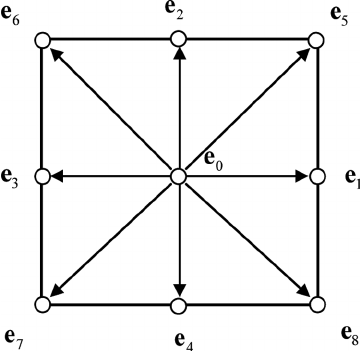
\includegraphics[width=0.3\linewidth]{Resources/Images/d2q9.png}
  \caption{2D LBM model using 9 particles. (D2Q9)}
  \label{fig:d2q9}
\end{figure}

\begin{figure}[H]
\centering
  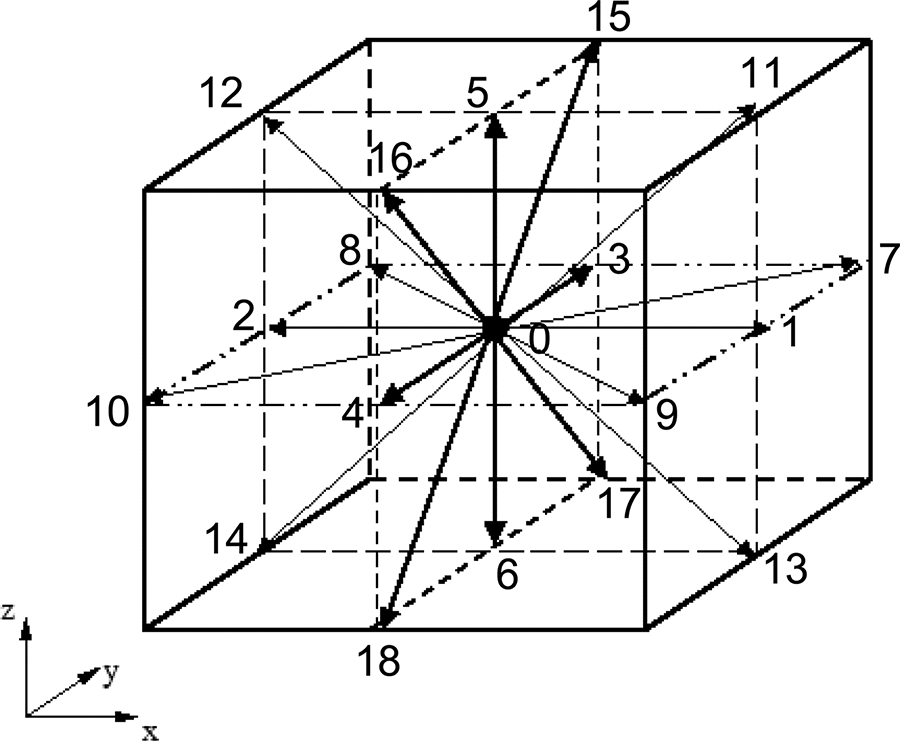
\includegraphics[width=0.3\linewidth]{Resources/Images/d3q19.png}
  \caption{3D LBM model using 19 particles. (D3Q19)}
  \label{fig:d3q19}
\end{figure}

\par
This way we can reap the advantages of both the macro and microscale approaches without the need of high end computers \cite{lbm_springer}. Since communications between nodes are very limited, LBM also offers the possibility of employing parallel computing to achieve the solution in even faster times.

\subsection{Multiphase flow}
Multiphase flows represent the simultaneous flow of materials in different states (phases). As such, multiphase flows have an enormous spectrum of representation and stand for interactions between gas/solid flows, liquid/solid flows or even liquid/liquid flows with different chemical properties \cite{multiphase}.\par
These simulations present challenging problems because of inherent difficulties during modelling and the importance of engineering applications. However, the Lattice Boltzmann method provides an alternative for these simulations due to it's relative simplicity when compared with traditional Navier-Stokes equation \cite{chenDoolenMP}.
\par These flows have several applications in the scientific and industrial community, ranging from pourous media fluid interactions \cite{pourous} to flows containing gas bubbles dispersed in liquids \cite{gasBubble}. Furthermore, almost every processing technology must take multiphase flows into account, including cavitating pumps, papermaking and many others \cite{multiphase}.
\par Several implementation strategies exist for Multiphase flows, however, for the purpose of this thesis, we will first follow the simple ''two-color'' approach first proposed by Gunstensen et al \cite{gunstensen} \textcolor{red}{This is wrong, refer to RK. Also, explain the history and how to method was developed}.


\section{High Performance Computing}
As humanity evolves, so too does our desire for expanding previous unobtainable goals. As computer technology kept progressing further and further, we soon realised that some problems simply took too many resources to be completed.\par
Figure \ref{fig:moore} shows the evolution of computing power over the past 120 years. Moore's Law states that ''processor speeds, or overall processing power for computers will double every two years'' \cite{moore}. Note that the last 7 most recent data points are NVIDIA GPUs.

\begin{figure}[H]
\centering
  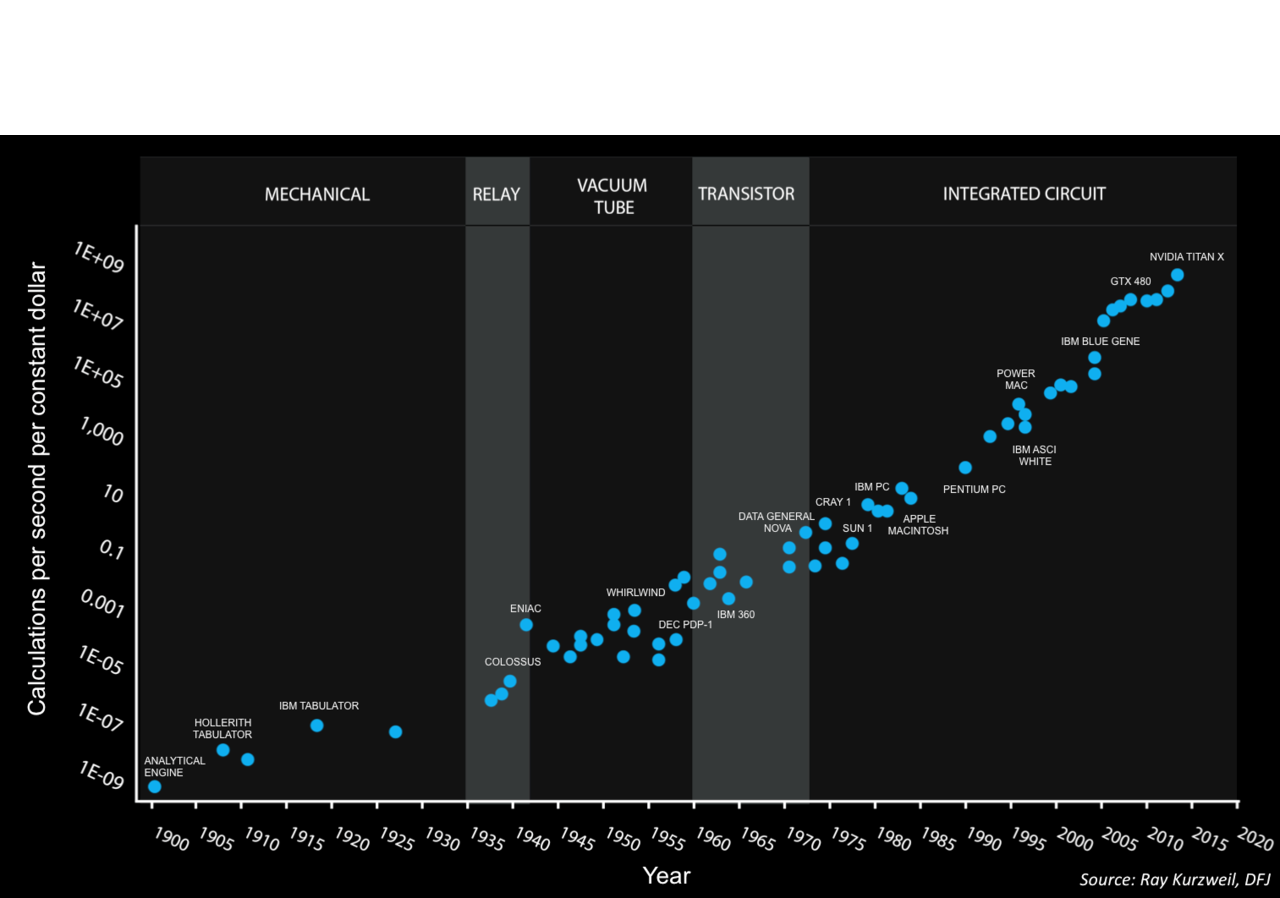
\includegraphics[width=0.6\linewidth]{Resources/Images/moore120.png}
  \caption{Moore's law over 120 years}
  \label{fig:moore}
\end{figure}

However, this evolution in computational power could only be achieved by combining CPU cores together.
So what if we focused our efforts in splitting the workload, effectively using the multiple cores available to produce a solution?\par
High performance computing (HPC) comes from the harnessing of computer power to deliver a much higher performance that one could not obtain from a typical computer. To this end, we can talk of HPC as being a collection of computer resources, all of them working simultaneously to achieve a solution of the same problem. Problems that could otherwise take weeks, months or even years can now be solved in minutes, hours or days under these powerful devices. However, different parallelisation strategies for splitting the workload emerge, depending on the underlying hardware. \par
It is also important to understand that parallel computing is achieved with the help of processors that will execute different calculations or processes simultaneously. To measure the parallelisation's efficiency, it is worth introducing the term Speed-up. The Speed-up is the ratio of the execution time of the parallel algorithm on a single processor with the execution time of the parallel algorithm on P processors \cite{irenehpc}. However, Amdahl's law states that ''in parallelization, if P is the proportion of a system or program that can be made parallel (...), then the maximum speed-up that can be achieved using N number of processors is $\frac{1}{\left(1-P\right)+\frac{P}{N}}$'' \cite{amdahl}. This means that our parallelisation efforts are limited by the amount of work that can be parallelised and, theoretically, should follow the distribution represented in Figure \ref{fig:amdahl}. 

\begin{figure}[H]
\centering
  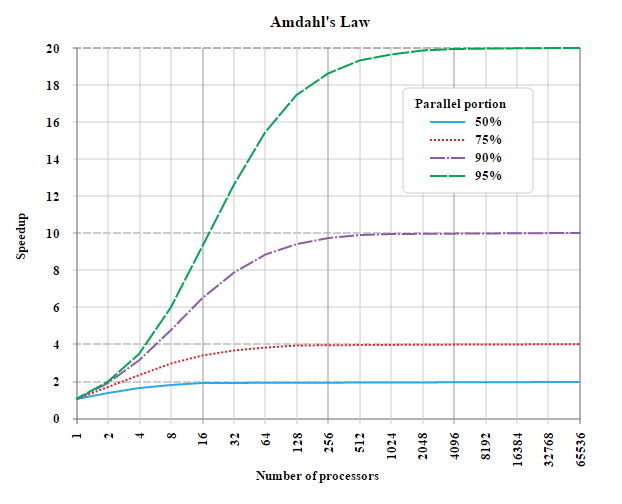
\includegraphics[width=0.6\linewidth]{Resources/Images/amdahl.png}
  \caption{A graphical representation of Amdahl's law}
  \label{fig:amdahl}
\end{figure}

\subsection{Distributed memory}
Following a distributed memory architecture for parallel computing means that each processor will have it's own independent local memory. In these systems, all the work that one process executes remains local to it, without interfering with the address space of all other processors. Hence, to solve meaningful computations, a communication network needs to be established in order for processes to share data with each other. Such is the case of the Message Passing Interface (MPI).\par
This means that this architecture is very scalable: with each processor being added to the system the size of the total memory increases. Also, each processor will be able to access it's own memory rapidly and without interference, reducing the usual constraint of memory access penalties.
\par However, this type of system requires a higher degree of skill from the programmer. The programmer will be the one responsible for most of the details of memory passing between processors and will need to ensure that no race conditions or deadlocks arise from the data communication. Also, whenever data from another processor is needed, the latency of the bandwidth in the network will introduce a heavy time penalty to the computations, as this data will need to be communicated before computations can be performed over it.
\subsection{Shared memory}
In a shared memory architecture, each processor is able to access all memory as global address space. This means that data can be handled seamlessly between processors, making programs easy to read and easy to write. An example of this model can be the Open Multi-Processing (OpenMP) API, which supports shared memory multiprocessing programming in C, C++ and Fortran. In this architecture, processors can operate independently while having access to the same memory resource pool as all other processors. Therefore, changes in the data handled by one process is visible and updated for all others. \par
This means that the programmer can have a user-friendly environment while working on his/her algorithm. All details concerning data flow between processes are abstracted, making this model very beneficial for users with little to no background in parallel programming. Also, the data being shared between processors is fast and uniform, making the penalties of memory access of this shared data less penalizing than in the distributed memory model.
\par However, this architecture presents little memory scalability, since adding more CPUs will increase the traffic of the shared memory path. Also, the programmer will have to pay close attention to memory access so as to prevent memory violation and ensure a correct synchronization of the access to the global adress space.

\subsection{GPGPU}

General Purpose computing on Graphical Processing Units stands for the use of Graphics Processing unit (GPU) to perform computations on applications normally performed by the CPU. One of the main advantages of using this approach is the amount of cores that a single GPU has. While a typical desktop CPU has up to 4 cores, a GPU can have thousands of cores, allowing users to take advantage of its massively parallel architecture. GPUs can now solve problems that were traditionally solved by the CPU. This is a big improvement, since GPUs are cheaper to acquire and more powerful than CPUs.\par
	NVIDIA then developed CUDA. CUDA code allows programmers to take advantage of GPUs by employing a unified shader pipeline under the familiar C language \cite{cuda_by_example}. Users were no longer required to have specific knowledge of OpenGL or DirectX and could now perform general computations (rather than graphic-specific computations) whilst benefiting from the massive computational powered offered by GPUs. 
	\par Programmers could now use the macros defined by CUDA to harness the full power of the GPU with a relatively small learning curve. If the user is already familiar with C language, then he can pick up on the details of the framework quickly. While this may seem like a big improvement, almost nothing comes without some disadvantages. CUDA can be excessively complicated to those unfamiliar with parallel programming. Although it offers the possibility of competing with several CPUs linked together, to optimise the kernel calls (device specific functions) takes a big attention to details and some knowledge on how the underlying hardware works. Users should not take this approach light-heartedly as they can easily become encumbered with work when compared to a simpler to use framework (such as OpenMP).  

\section{Previous parallelisation works}
This thesis is a continuation of work that started some years ago in Cranfield University. As such, the work from the previous students needs to be analysed. \par
In 2014, Tamás Józsa and Máté Szőke, adapted two different in-house C and C++ codes into one single C code unifying the advantages of each one of the two original codes \cite{jozsa_thesis,szoke_thesis}. Józsa then parallelised the critical parts of the C code using CUDA and ran tests on the Fermi GPU Cluster from Cranfield, achieving a three times speed-up in general, with a peak of 15 times speed-up \cite{jozsa_thesis}. \par
Szőke proposes a CPU parallelisation approach using Unified Parallel C, which is a Partitioned Global Address Space language\cite{szoke_thesis}. This means that it is possible to use shared memory to compute the solution. However, the author verified that a local memory-based approach (like MPI) provided the best results. He also compared the results obtained with the ones obtained by Józsa on the CUDA approach. They found that to achieve the same speed-up as that of a single GPU card, one needs an entire workstation (16 threads in the case of Astral) \cite{szoke_thesis}.\par
In 2015, Ádám Koleszár continued the work and further optimised the parallel version of the LBM method using CUDA \cite{koleszar_thesis}. He did an excellent job, resulting in a 10 times faster execution than the previous 2D parallel solver, which means that his new optimised code was 30 times faster than the original, in-house, serial solver.\par
Finally, in 2016, Maciej Kubat proposed a new version of the LBM solver.Firstly he converts the 2D parallel solver to a 3D parallel solver which entailed a major re-engineering of the code, from data containers to logic cycles \cite{maciej_thesis}. After first trying for a direct adaptation, he found that his code was too slow to produce meaningful solutions. After optimising his own code he was able to reach an almost one hundred times speed-up.
However, Kubat states that a lot can be done to improve his code, from boundary conditions to code readability and maintainability. 
\chapter{Methodology}
\section{Lattice Boltzmann Method}
The Lattice Boltzmann method is a mesoscopic approach to solve several fluid dynamics problems, \textcolor{red}{as stated in Section}. It relies on a statistical description of the system via a distribution function $f$. This distribution function is responsible for predicting the number of molecules at a certain time, positioned between 2 points and with velocities between 2 values. This function is used in combination with a collision operator $\Omega$ and, with no external force being applied, represent the Boltzmann equation as
\begin{equation}\label{eq:boltzEq}
\frac{\partial f}{\partial t} + c \nabla f = \Omega
\end{equation}
giving us an advection equation. 
However, Eq. \ref{eq:boltzEq} is difficult to solve by itself. To offset this difficulty we need to approximate the collision operator with a simpler operator that will not introduce a significant error in the final solution. After solving this collision step, we then need to propagate the changes in each cell onto to their neighbours (streaming). We then solve boundary interactions within the nodes affected by the boundary spaces of the problem and finally we update the macroscopic values. These values will be fed into the collision step again where the process will repeat itself until the solution converges/diverges or the final number of iterations is reached.
\subsection{Discretization}
Before starting with the collision step, we must first discretize the domain into a mesh composed of various cells. Each of these cells will in turn affect and be affected by other cells, depending on the chosen speed model, as stated in Section \ref{sec:lbmLit}. As such, we will use a 2DQ9 arrangement for the 2D problems and a 3DQ19, which roughly translates into each cell interacting with another 8 or 18 cells (neighbours), depending on the problem's dimension.
\subsection{Collision}
There are a few collision models capable of approximating the collision operator $\Omega$, such as the BGKW \textcolor{red}{cite}, the TRT \textcolor{red}{cite} and the MRT  \textcolor{red}{cite}. However, for the purpose of this thesis, we will focus solely on the BGKW model as this will be the approximation used by the Multiphase model. \par
In the BGKW model, we can use the following equation to approximate $\Omega$
\begin{equation}\label{eq:bgkwEq}
\Omega = \omega \left( f^{eq} - f\right) = \frac{1}{\tau}\left( f^{eq} - f\right)
\end{equation}
where $\omega$ represents the collision frequency and $\tau$ stands for the relaxation factor. $f^{eq}$ represents the local equilibrium of the distribution function, which is known as the Maxwell-Boltzmann distribution function. Now, we can use Eq. \ref{eq:bgkwEq} in the discretized Boltzmann equation to obtain
\begin{equation}
f_i = \omega f^{eq}_i + (1 - \omega)f_i%\frac{\partial f_i}{\partial t} + c_i \nabla f_i = \frac{1}{\tau}\left( f^{eq}_i - f_i\right)
\end{equation}
which will be valid when following specific directions.
\subsection{Streaming}\label{sec:streaming}
After each node finishes calculating the changes brought on by the collision with other nodes, it is necessary to pass this information onto each neighbour. This streaming will take into account the directions imposed by the speed model. Figure \ref{fig:streaming} demonstrates how this step of the method works for the two dimension problem type.

\begin{figure}[H]
	\centering
	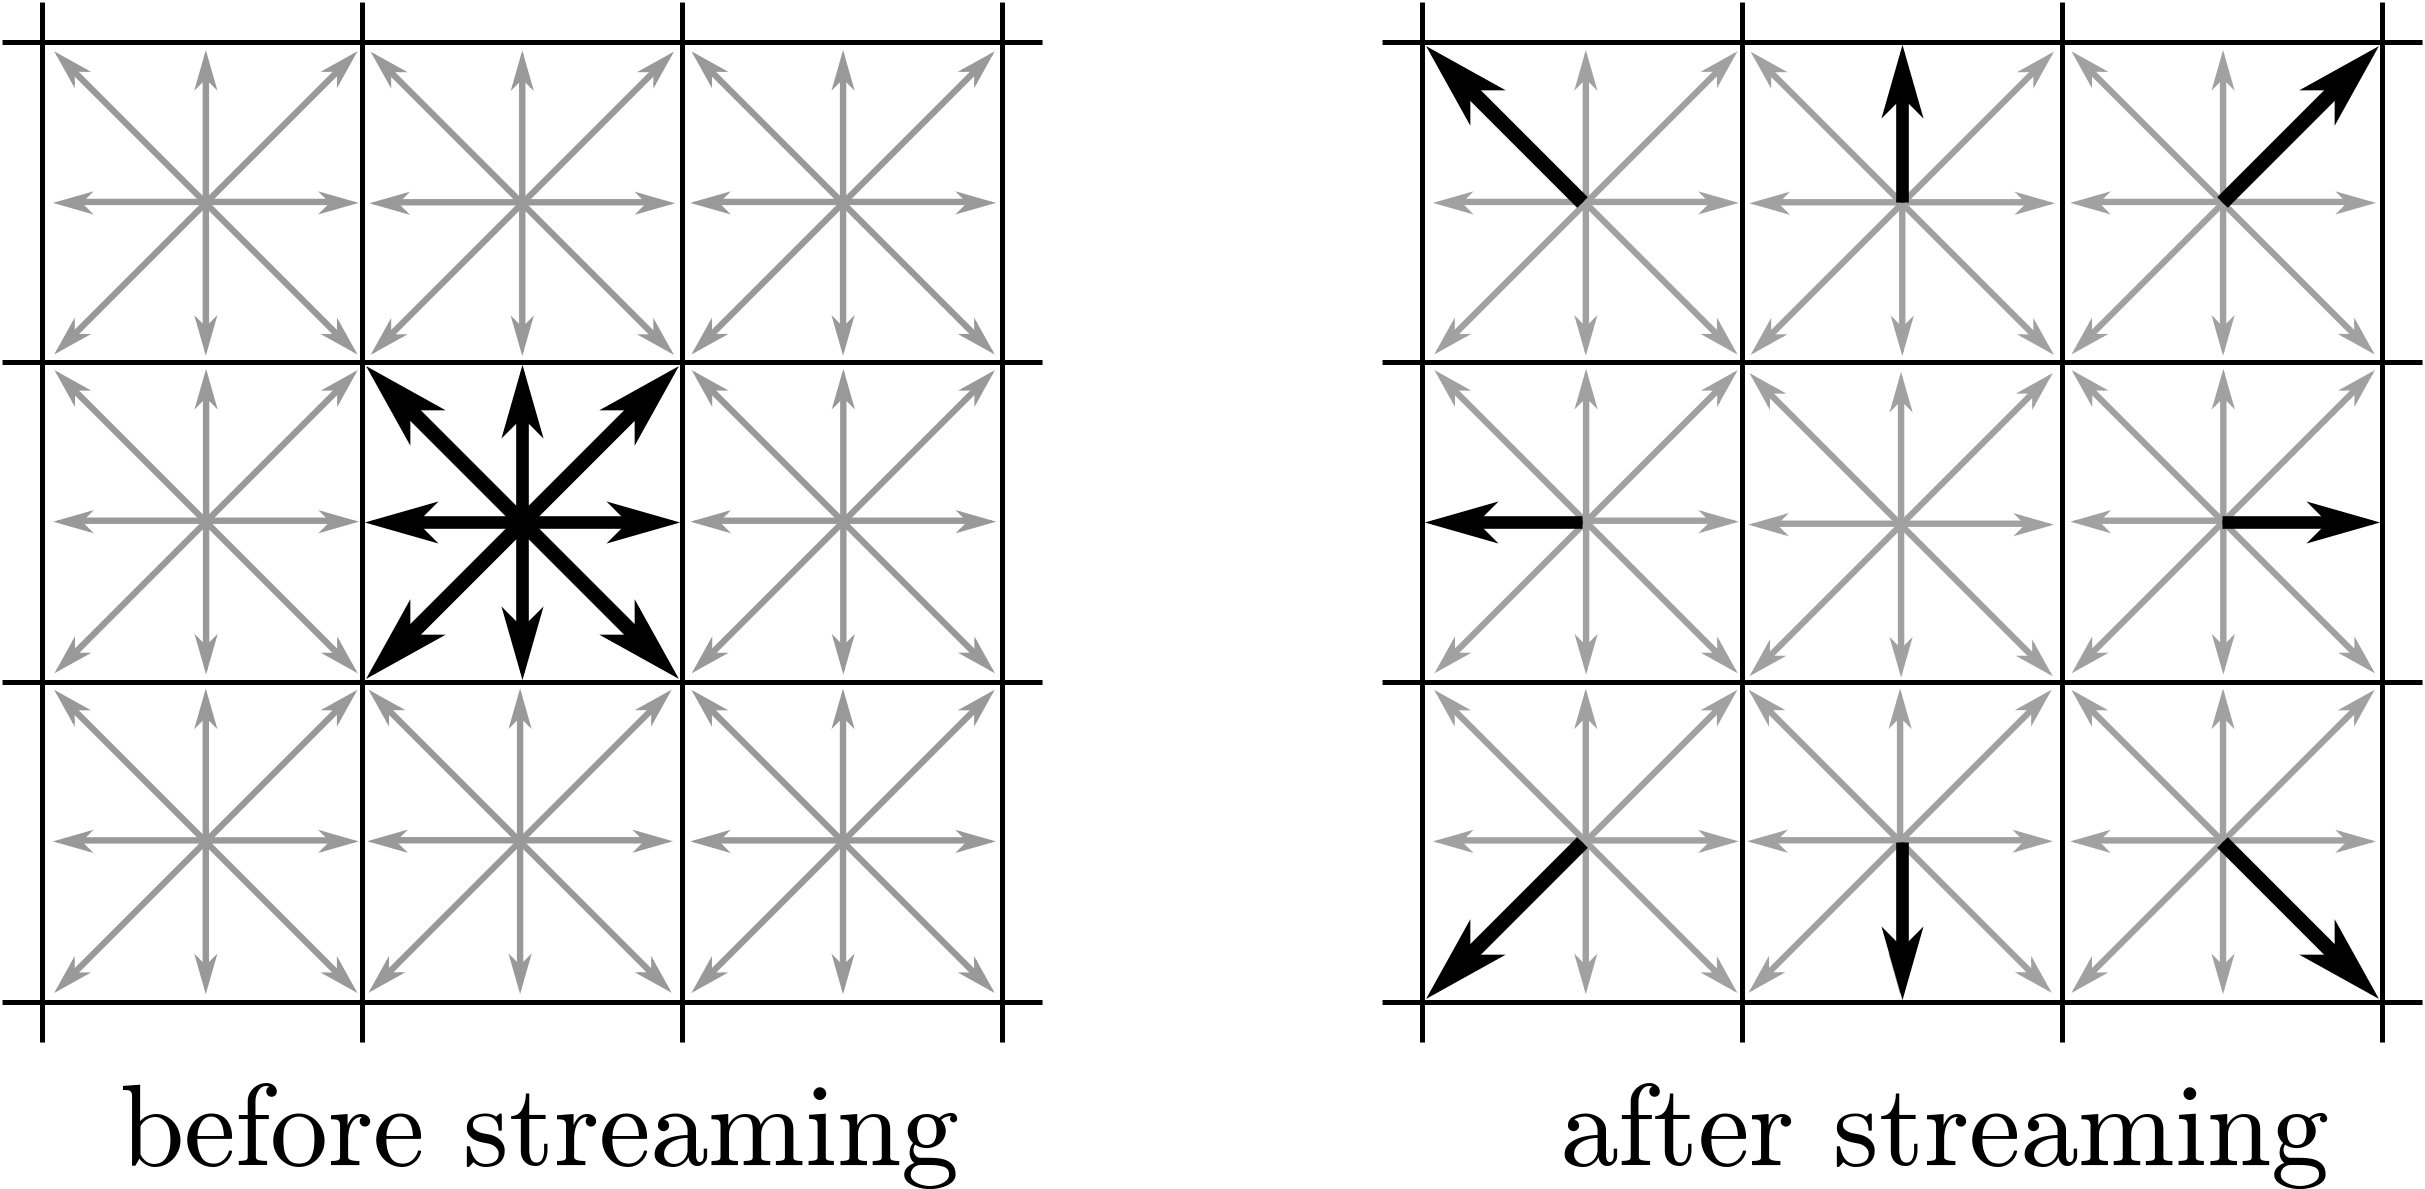
\includegraphics[width=0.8\linewidth]{Resources/Images/streaming.png}
	\caption{Streaming step following a 2DQ9 model.}
	\label{fig:streaming}
\end{figure}

For 3D problems the streaming step follows the same strategy.
\subsection{Boundary update}\label{sec:boundary}
After each node updates their neighbour, the nodes located on the boundaries of the problem need to be updated depending on the boundary condition applied to them. Again, there are quite a few boundary conditions implemented in the in-house solver. However, the author will only go into detail in the boundary conditions used by the new Multiphase model.\par
\subsubsection{Wall}
	These boundary conditions are implemented with a bounce-back effect, where particles that are incoming into the solid wall bounce back into the domain. Applying the laws of conservation of mass and momentum, a particle incoming into the southern direction of the domain leads to  
	\begin{equation*}
		\begin{aligned}
			f_2 = f_4 \\
			f_5 = f_7 \\
			f_6 = f_8
		\end{aligned}
	\end{equation*}
	\subsubsection{Periodic boundary conditions} 
	With these boundaries, particles that exit the domain on one side will enter the domain on the opposite, creating an infinite corridor between opposite sides. As such, if a particle reaches the north boundary, their distribution function will be updated as follows
	\begin{equation*}
		\begin{aligned}
			f_4^N = f_4^S \\
			f_7^N = f_7^S \\
			f_8^N = f_8^S
		\end{aligned}
	\end{equation*}
	\subsubsection{Inlet}
	 Zou and He \textcolor{red}{cite} proposed a method for solving these boundary conditions. In this case, the boundary simulates a fluid flow entering the domain with a certain velocity. Applying the proposed equations to the BGKW model on a cell located in the north boundary yields:
	\begin{equation*}
		\begin{aligned}
			\rho &= \frac{1}{1+v} * \left(f_1 + f_3 + 2 * \left(f_2 + f_5 + f_6\right)\right) \\
			f_4 &= f_2 - \frac{2}{3}\rho v \\
			f_7 &= f_5 + \frac{1}{2}\left(f_1 - f_3\right) - \frac{1}{6}\left(\rho v\right) - \frac{1}{2}\left(\rho u\right) \\
			f_8 &= f_6 + \frac{1}{2}\left(f_1 - f_3\right) - \frac{1}{6}\left(\rho v\right) + \frac{1}{2}\left(\rho u\right)
		\end{aligned}
	\end{equation*}
\subsection{Macro-variables update}\label{sec:mpUpd}
Finally, after updating the distribution function of every cell in the domain, we can update the macroscopic variables $\rho$, $u$ and $v$.
From Eq. \ref{eq:boltzEq}, we can define the macroscopic values for density and velocity as
\begin{equation}\label{eq:densityUp}
\rho (r,t) = \int  mf(r,c,t)dc
\end{equation}
\begin{equation}\label{eq:velocityUp}
\rho (r,t) u(r,t) = \int  mcf(r,c,t)dc
\end{equation}
where $m$ represents the molecular mass.
\section{Color Gradient Model}\label{sec:cgModel}
Models implementing multiphase flows for the Lattice Boltzmann method can generally be classified into several different categories. For the purpose of this thesis, we will focus on the Rothman-Keller methods, specifically on the model proposed by Reis and Phillips \textcolor{red}{cite}, modified using Latva-Kokko's recoloring operator, as proposed by Leclaire et al. \textcolor{red}{cite leclaire}. \par
In this model, two immiscible fluids are simulated under the LBM, a red fluid and a blue fluid, that only interact with each other in the interface between them. These fluids are associated to their own distribution functions, which implies that the total memory used by the in-house solver is likely to increase. Furthermore, the collision step will need to be created from scratch since this step introduces two new operators, while the standard collision step will also suffer some changes to account for the two fluids. \par
The fluid's distribution function now becomes
\begin{equation}\label{eq:cgDistrib}
f_{i}^{k}\left(x+c_i, t+1\right) = f_{i}^{k}\left(x,t\right) + \Omega_i^{k}
\end{equation}
where $k$ stands for the fluid, either red or blue.$\Omega_i^{k}$ is the result of the combination of the 3 sub-steps present in the new collision step and is given by
\begin{equation}\label{eq:cgColl}
\Omega_i^{k} = \left(\Omega_i^{k}\right)_{\left(3\right)} \left(\left(\Omega_i^{k}\right)_{\left(1\right)} + \left(\Omega_i^{k}\right)_{\left(2\right)}\right)
\end{equation}
\subsection{Single-phase collision operator}
The first sub-step is similar to the collision operator used in the standard BGKW model, introduced in Eq. \ref{eq:bgkwEq}. However, a new operator, $\phi$ is introduced in the calculation of the local equilibrium distribution function. 
\begin{equation}\label{eq:newFEQ}
f_i^{k\left(eq\right)} = \rho_k\left(\phi_i^k + W_i\left(3c_i \cdot u + \frac{9}{2}\left(c_i \cdot u\right)^2 - \frac{3}{2}u^2 \right)\right)
\end{equation}
where $\phi_i^k$ is given by 
\begin{itemize}
	\item $\alpha_k$ for $i = 0$
	\item $\frac{\left(1-\alpha_k\right)}{5}$ for $i = {1,2,3,4}$
	\item $\frac{\left(1-\alpha_k\right)}{20}$ for $i = {5,6,7,8}$
\end{itemize}
\subsection{Perturbation operator}
After computing the single-phase collision operator we need to add the result of the perturbation operator before passing it on to the recoloring sub-step. This is where we simulate the surface tension between the fluids and ensure that pressure difference is in equilibrium.\par
First, we must calculate the color gradient term, which is defined by
\begin{equation}\label{eq:colorGrad}
F = \sum_i c_i \left(\rho_r\left(x+c_i\right) - \rho_B\left(x+c_i\right)\right)
\end{equation}
which is 4th order accurate. Then, we include $F$ in the calculation of the perturbation term, defined by
\begin{equation}\label{eq:pert}
\left(\Omega_i^{k}\right)_{\left(2\right)}\left(F_i^k\right) = F_i^k + \frac{A_k}{2}\norm{F}\left(W_i\frac{\left(F\cdot c_i\right)^2}{\norm{F}^2} - B_i\right)
\end{equation}
\subsection{Recoloring operator}
The last step in the collision step is calculating the recoloring operator. This operator guarantees that the fluids remain immiscible and also controls the amount of a fluid sent to it's corresponding region. The operator can be defined as
\begin{equation}
\left(\Omega_i^{k}\right)_{\left(3\right)}\left(F_i^k\right) = \frac{\rho_k}{\rho}F_i + \beta\frac{\rho_r \rho_b}{\rho^2}\cos \left(\phi_i\right)\sum_k F_i^{k\left(eq\right)}\left(\rho_k,0,\alpha_k\right)
\end{equation}
where $\beta$ is a free parameter between 0 and 1 that influences the thickness of the interface and $\cos \left(\phi_i\right)$ is the cosine of the angle between the color gradient $F$ and the direction $c$.
\subsection{Streaming and Boundary conditions}
The streaming and boundary conditions in this model are analogous to the ones used in the LBM method, as defined in Sections \ref{sec:streaming} and \ref{sec:boundary}. To compute them, we simply need to repeat these steps for the distribution function of each fluid.
\subsection{Macro-variables update}
This step is also similar to the one defined in Section \ref{sec:mpUpd}. The main difference is that $\rho$ is the result of the sum of the densities of each fluid and $F_i$ is also the sum of the distribution functions of each fluid. 
\section{Meshes}
For the LBM in-house solver we need to prepare structured meshes capable of representing the domain. These meshes allow us to discretize the functions and solve them according to the representation of space. Each mesh is composed of equidistant small spaces that represent the cells used in the equations. To this end, software capable of generating meshes is needed, that can both create the mesh according to the number of nodes required and specify the type of boundary conditions to be used. G. Abbruzzese developed software capable of generating meshes with these requirements \textcolor{red}{cite} which has been used in the previous thesis over the LBM in-house solver. \par
However, only the 3D lattice generator still exists, which means that we are restricted to the 2D meshes that already exist. Luckily, these meshes are sufficient to simulate the requirements of all of the proposed test cases. The boundaries however will need to be hard-coded to match the initial requirements and to adequately simulate the 2D test cases.
\subsection{Used meshes}
The test cases for the Color Gradient model are based on a simple square for 2D or a cube for 3D problems. However, the boundaries are specific to each case. All of them use periodic boundaries on the East and West directions and most of them also use them for the North and South directions, the exception being for the Couette flow where the North boundary is an Inlet and the South boundary acts a solid wall.
\section{CUDA programming}
As stated before, CUDA is a parallel programming platform introduced by NVIDIA. One of it's most appealing features is the fact that it is integrated into the well known programming languages C/C++, making it easy for programmers to start developing parallel code in a familiar environment. However, there are some details that one must know before being able to take benefit of the computational capabilities of GPUs. Note that the host is referring to the CPU and the device is referring to the GPU.
\subsection{Thread arrangement}
As is the case with several other parallel programming platforms, CUDA's base parallel agents are threads. CUDA allows for a massive number of threads running concurrently. However, accessing each thread is not as straightforward as one would hope. Figure \ref{fig:threads} show how threads are organized inside CUDA's memory model.

\begin{figure}[H]
	\centering
	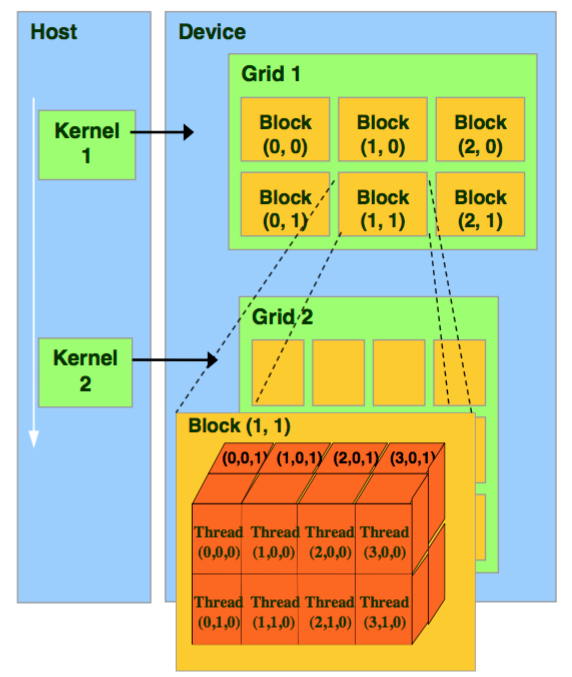
\includegraphics[width=0.6\linewidth]{Resources/Images/threadmapping.png}
	\caption{Thread arrangement in CUDA platform.}
	\label{fig:threads}
\end{figure}

Threads are organized into blocks and blocks are organized in the grid. Both the grid of blocks and the blocks themselves can be of 1, 2 or 3 dimensions. CUDA provides a very useful way of obtaining the index of each thread. We can easily obtain the thread's index inside the block as well as the block's index in the grid. However, some math is needed to obtain the thread's global index, which is very useful for memory management, such as access to an array's element. Fortunately, this is an easy task since we can access all the needed information with threadIdx, blockDim, blockIdx and gridDim.

\subsection{Memory structures}
Since CUDA code runs on GPUs, it is worth showing what the internal architecture of a NVIDIA GPU looks like. 
\begin{figure}[H]
	\centering
	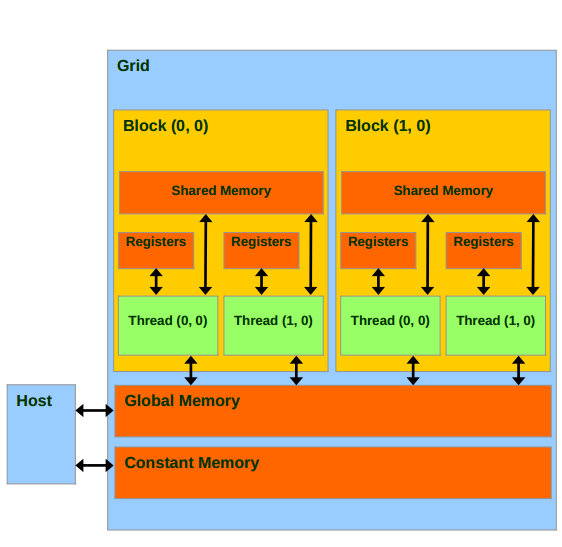
\includegraphics[width=0.8\linewidth]{Resources/Images/cudaMemory.png}
	\caption{Memory arrangement in CUDA compliant GPU.}
	\label{fig:memCuda}
\end{figure}

Figure \ref{fig:memCuda} shows 4 different types of memory available to each thread
\begin{itemize}
	\item Registers
	\item Shared memory
	\item Global memory
	\item Constant memory
\end{itemize}

There is also one more memory type, texture memory. However, this memory type will not be used in the scope of this thesis, so the author will not go into detail about them.
\subsubsection{Registers}
Registers are the fastest type of memory available to a thread. Each thread's register is only visible to itself and so every variable using this type of memory is visible only to the thread. This means that it is not possible to use data directly from the host on these structures. Also, this data is non-transferable between threads. \par Registers work just like local memory for each thread, the difference is that local memory is comparable to global memory in terms of speed since it is not allocated directly on the GPU chip but is instead an abstraction of global memory. Local memory will only be used if the compiler determines that the thread's register size is not large enough to hold the thread's local memory.
\subsubsection{Shared memory} 
Shared memory is the second fastest type of memory available to a thread. As opposed to registers, shared memory is, as the name suggests, shared between threads residing in the same block. This means that we can have threads cooperating with each other when using this type of memory. However, memory access needs to be properly managed, otherwise degrading memory access speed when bank conflicts occur. Bank conflicts means that two or more threads are trying to access the same memory address, and when this happens the memory access is serialized between the conflicting threads.\par
The nature of this memory makes it an excellent candidate for cases where threads require information from other threads to continue with their work, for example in a matrix vector multiplication. In these cases, a proper management of shared memory within the block can greatly boost the algorithms performance. As such, this a memory structure that should be used whenever threads require cooperation since with no bank conflicts shared memory can reach the speed of register memory.
\subsubsection{Constant memory}
This a read-only type of memory that is stored in the cache, making access to it faster than global memory. This is the first memory type that can transfer data between the host and the device since before using in the device data needs to be properly initialized within the host code. Cached memory has the benefit that a single read can be broadcast to other 15 threads, and also that consecutive reads from the same address space will not incur any additional memory traffic \textcolor{red}{cite cuda}. However, we can only benefit from a performance gain when using constant memory if we pay attention to the warps inside a block, since the memory read is broadcast to a half-warp (more on this later).
\subsubsection{Global memory}
Finally, we reach the slowest yet most versatile memory in a CUDA compliant GPU. Global memory has, as the name suggests, a global scope, meaning that every thread inside the grid can access it, as is the case with constant memory. However, it is not limited to read-only access as all threads can also write data onto it. This is the only other data that can be transferred between host and device (apart from texture memory) but it has the disadvantage of being the slowest memory type. To boost performance, data in global memory will usually be read into a faster memory type like registers or shared memory before having computations performed over it.

\subsection{Warps}
A warp is a group of 32 threads inside a block. Each block, when it is created, is assigned to a Streaming Multiprocessor that contain 32 processing cores \textcolor{red}{cite webinar}. The threads inside a warp are truly concurrent, meaning that at a given time each thread will execute the same instruction concurrently (lock-step fashion). Therefore, warp-awareness is essential to write highly-optimised code \textcolor{red}{cite salvatore}. One must guarantee that each thread inside the warp will follow the same control path, otherwise risk wasting the full potential of the warps concurrency by achieving warp divergence.

\chapter{Results and Discussion}
\section{In-house LBM solver}
The implementation of a 3D multiphase flow using the Lattice Botzmann method will be based on an existing in-house code. As such, the first step in developing the new solver is to acquire a good understanding of how the previous solver works, specifically, it’s structure and organisation, it’s input and output data, it’s performance and it’s depending software (if any). Furthermore, the previous code needs to be validated so as to provide and accurate foundation for the project being developed. Without this validation, it would prove to be an arduous work to discover whether the new solver is behaving correctly.
\subsection{Code organisation}
After spending some time analysing the LBM solver and debugging some of the core features, I was able to obtain a generous understanding of how the existing code is organised and where most of the necessary algorithms are located. The solver itself was very well documented and most of the solver’s features were written in a very user-friendly way. Because of this good work from the authors of this solver, the following flow chart, Figure \ref{fig:codeFlow}, was able to be made in a relatively small amount of time, which helps to gain a general understanding of the solver.

\begin{figure}[H]
	\centering
	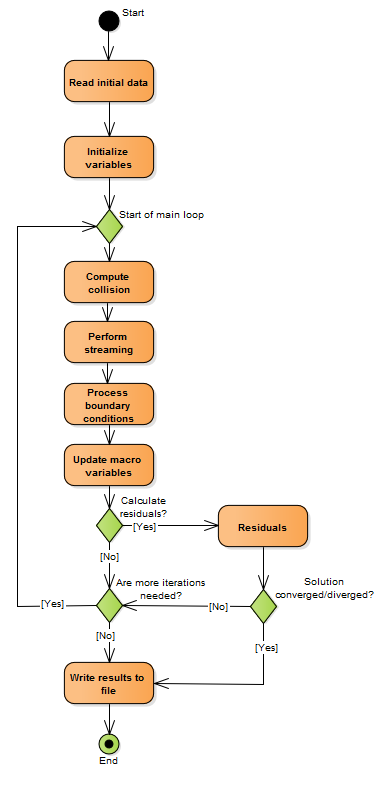
\includegraphics[width=0.5\linewidth]{Resources/Images/CodeFlowchart.png}
	\caption{A simplified flowchart of the solver's activity}
	\label{fig:codeFlow}
\end{figure}

The previous authors strived for a optimized and easy to use code. As such, the SetUpData.ini file contains all the information needed to build the problem to be solved. This file, combined with the mesh files that the user wishes to simulate, provide the initial step in running the solver. Note that external calculations need to be used to guarantee some aspects of the initial conditions, such as the Reynolds number.\par
Similarly, when the solver finishes computations, a Results folder is created containing information pertinent to the solution of the solver. These files include the final solution, the residuals, the run time, etc. The user also has the option of selecting which output format to produce the solution in (.vti, .dat or .csv).

\subsection{Data representation}
The original code mostly handles multidimensional arrays, following the same logic from the 2D solver onto the 3D version. As such, the arrays either store the macroscopic value of each node (h * m * n in 3D) or the coefficient for the microscopic values of each lattice (19 * h * m * n in 3D) . However, when using CUDA kernels, we will often have the need to copy data from the host (CPU) to the device (GPU), which can prove to be a tiring and inefficient task when dealing with 2, 3 or even 4 dimension arrays. To solve this problem, the previous authors flattened every array, which means that all arrays are represented as one dimensional arrays. Because of this, some calculations are required to access the desired index, \textcolor{red}{as demonstrated by Fig.}
\par These arrays are stored in a row-major fashion and the lattices are grouped together in 9 or 19 arrays, depending on the dimension of the problem, meaning that neighbours are separated from each other by m * n or h * m * n elements.

\subsection{Performance}
This thesis will be based on the work of previous Cranfield MSc students. As such, the received solver needs to be validated regarding the established performance in Kubat’s thesis \cite{maciej_thesis}. To this end, I generated the same meshes as the ones used in his thesis, specifically the lid driven cavity 128 and 256. \par
The lid driven cavity is a commonly used benchmark test for CFD solvers. It consists of a cube with a moving lid on the top which acts as the inlet for the flows. The numbers refer to the number of nodes in each direction, i.e. cavity 128 represents a 128x128x128 cube, resulting in 2097152 nodes.
\par
The final run-times of both meshes were very similar to the ones previously obtained, as shown in Figure \ref{fig:compareTimes}. Because of this, we can be sure that our version of the solver is the same as the final one used by the previous authors during their theses. \par

\begin{figure}[H]
	\centering
	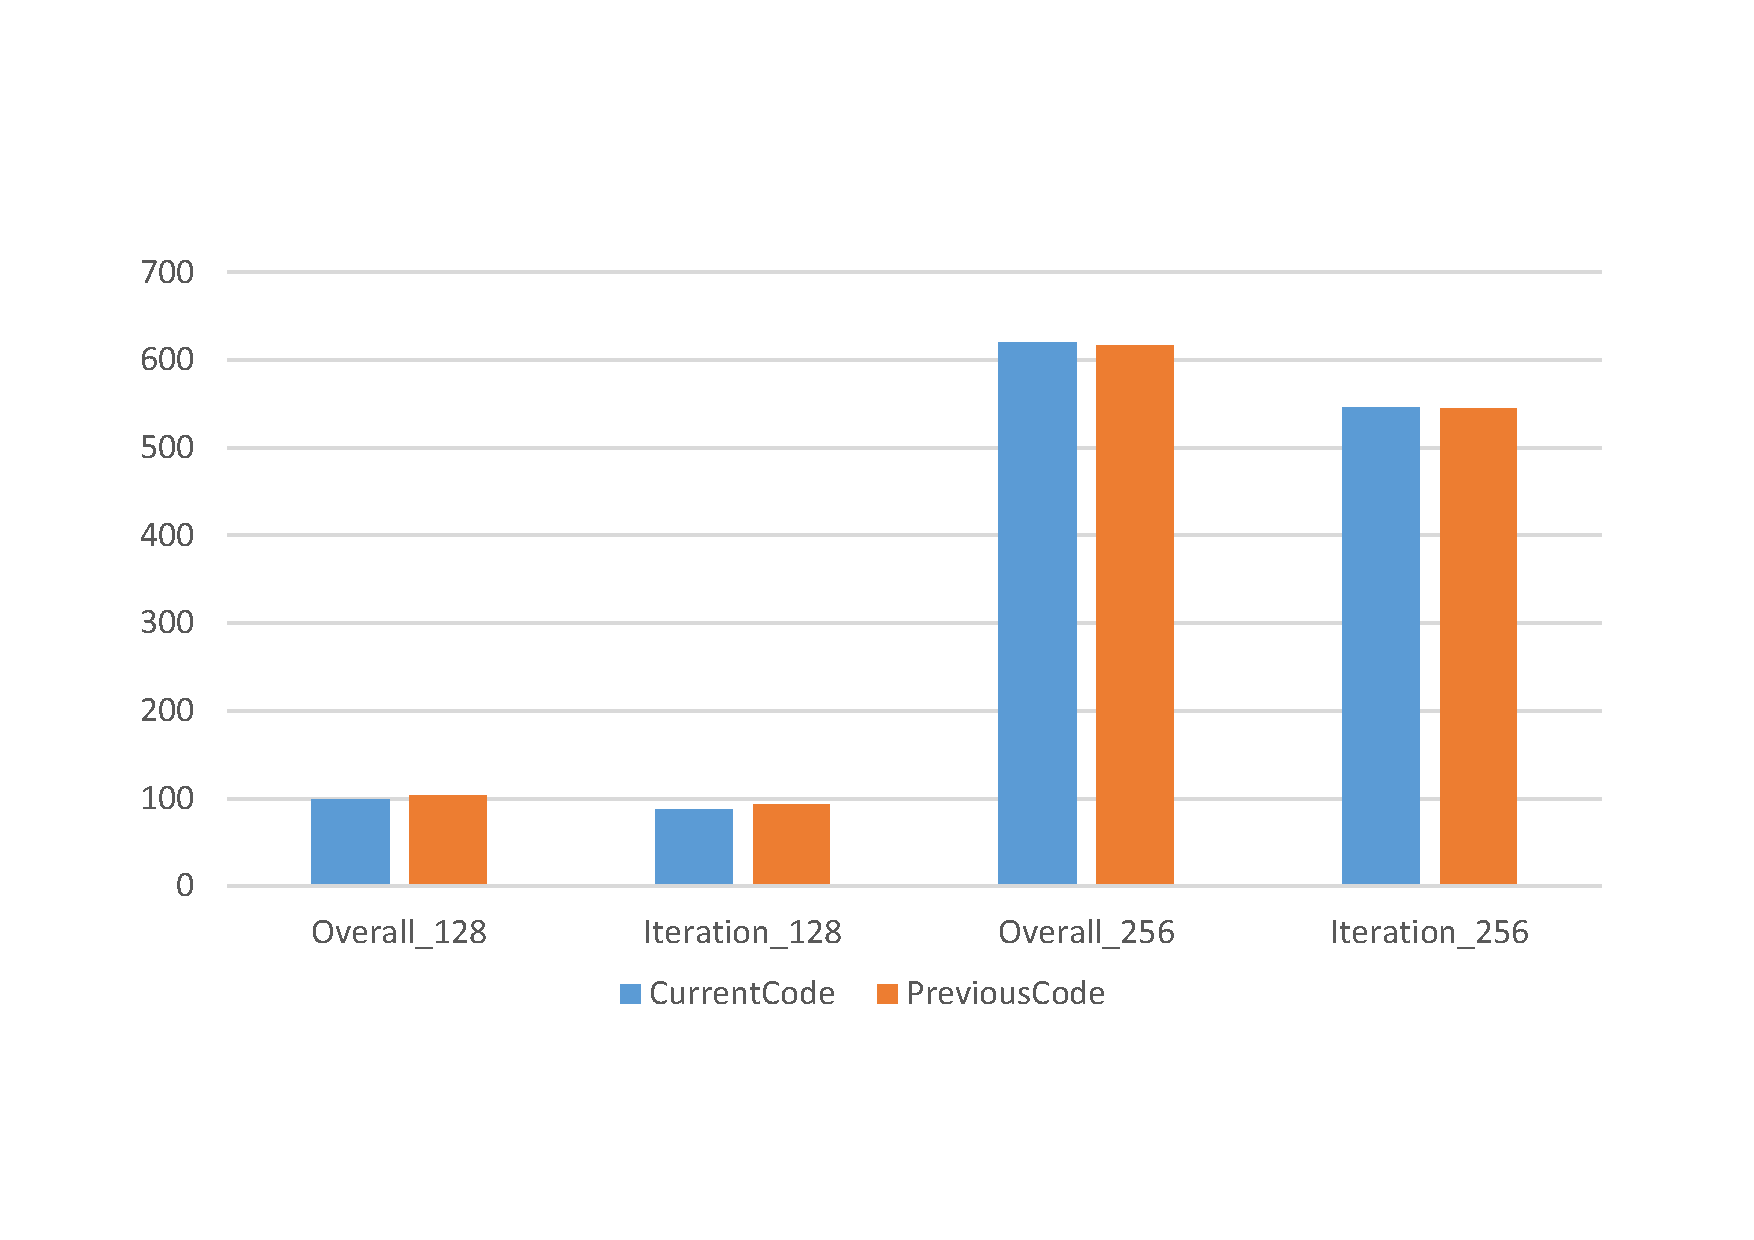
\includegraphics[width=0.9\linewidth]{Resources/Images/compareTimes.pdf}
	\caption{Runtime for Cavity\_128 and Cavity\_256}
	\label{fig:compareTimes}
\end{figure}


To gain a better understanding of the code, the solver’s run-times were profiled according to the main phases of the method. Figure \ref{fig:initialProfiling} shows that the solver spends about 40\% of it’s time calculating residuals. The residuals are used to check whether the solution has converged or diverged, making them a valuable method for potentially saving computation time (which in HPC centres means saving money). However, if the user is sure that the problem being solved needs to run for the specified iterations, he might be able to speed up the solver by not calculating the residuals, or even by specifying an interval of iterations before calculating residuals again.

\begin{figure}[H]
	\centering
	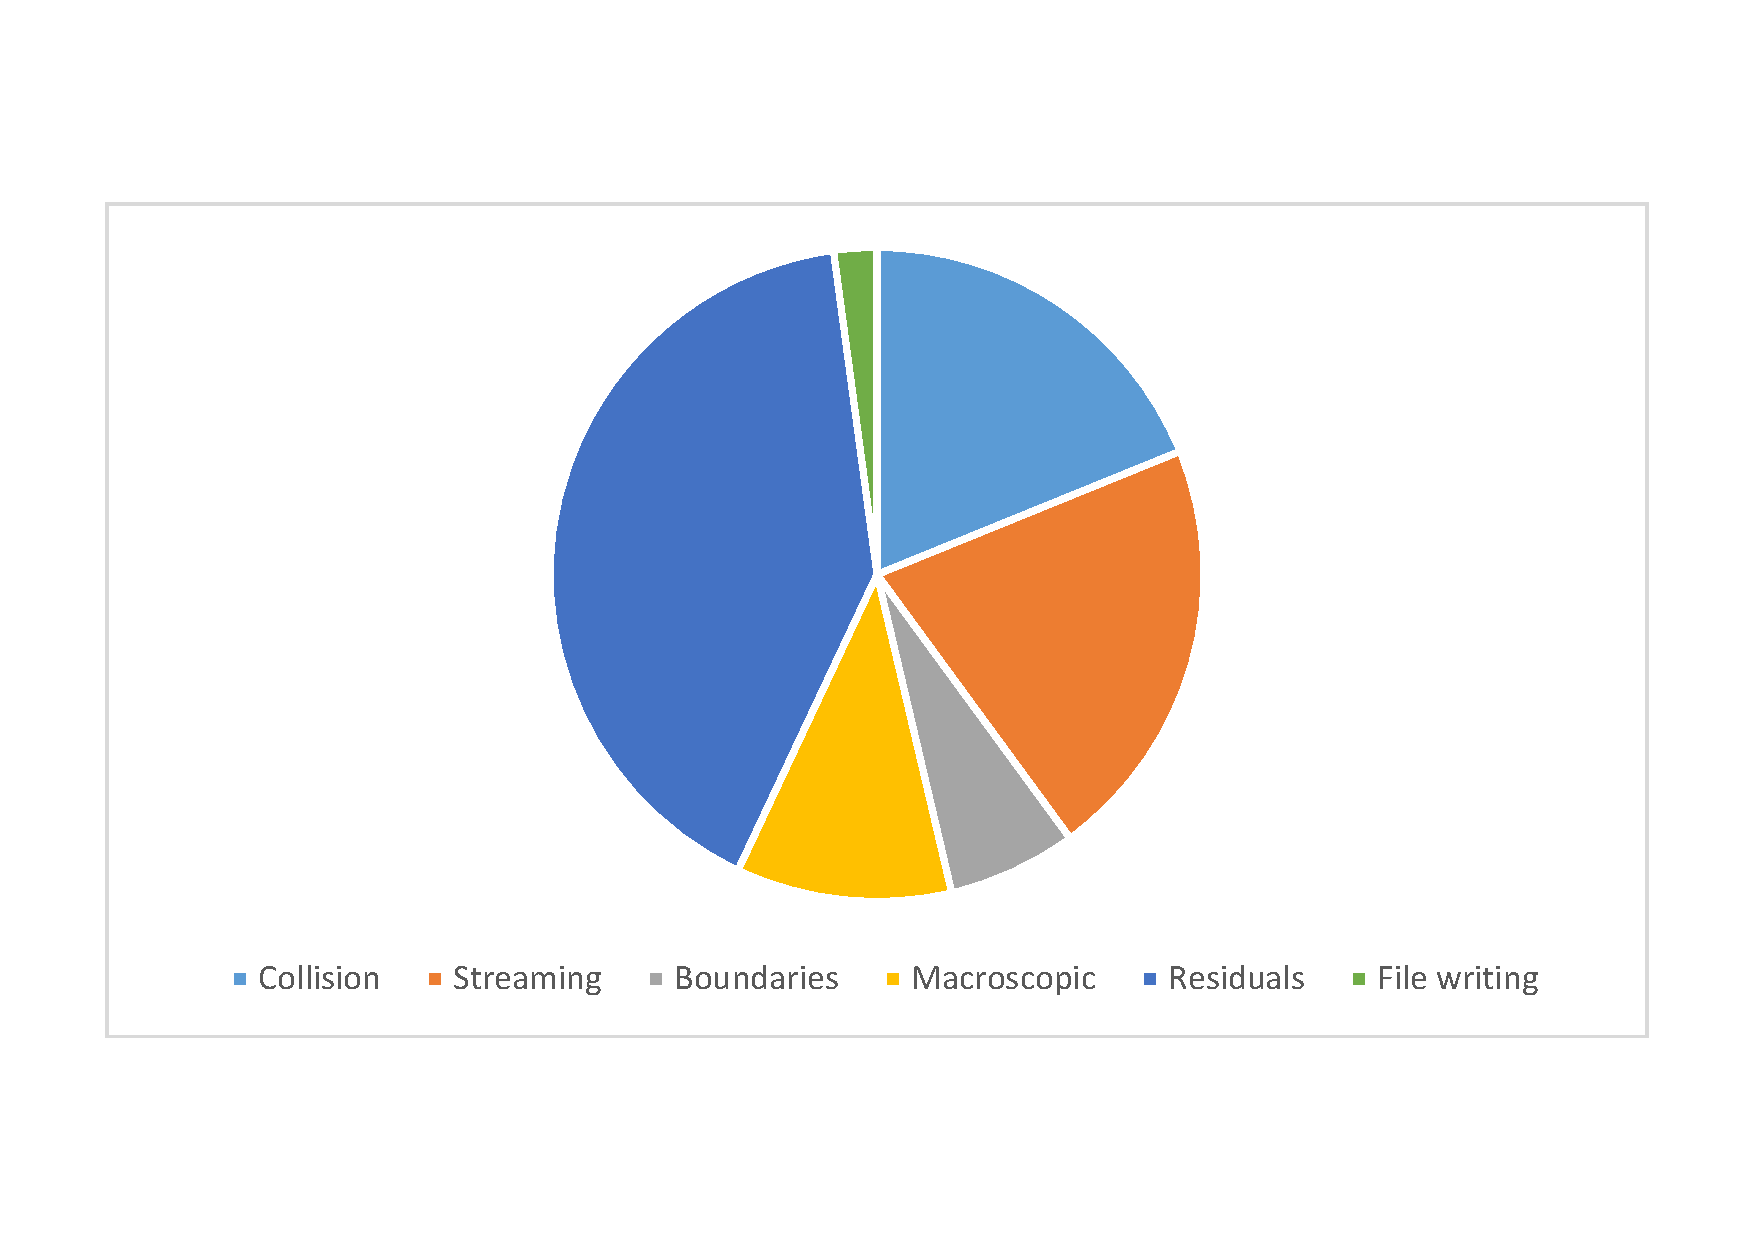
\includegraphics[width=0.9\linewidth]{Resources/Images/initialProfiling.pdf}
	\caption{Code profiling for the run-times of Cavity\_128 with MacroDiff residuals}
	\label{fig:initialProfiling}
\end{figure}

\par The remaining time is split between the collision, streaming and macroscopic values calculation, with boundary condition calculations and file writing occupying a less important slice of execution time. With this profiling, we now know which are the most critical parts of the software (residuals, collision and streaming) and can focus our efforts in optimising those areas when developing the method for multiphase flows.
\par Finally, the received solver was programmed to run with a 2D configuration in the kernel calls. Both the blocks per grid and threads per block are set up to run with an equal number of elements in the two directions. \textcolor{red}{The number of blocks is calculated dynamically with problem size in mind and sets 1 block per node.} However, the number of threads per block is declared statically with a value of 16x16. This means that the solver will use 16 threads in the x direction and another 16 in the y direction per block, meaning that each block uses 256 threads. To understand how this value affects the solver, I have benchmarked the solver using two more configurations for the Cavity\_128 and Cavity\_256 meshes.

\begin{figure}[H]
	\centering
	\begin{subfigure}{.49\textwidth}
		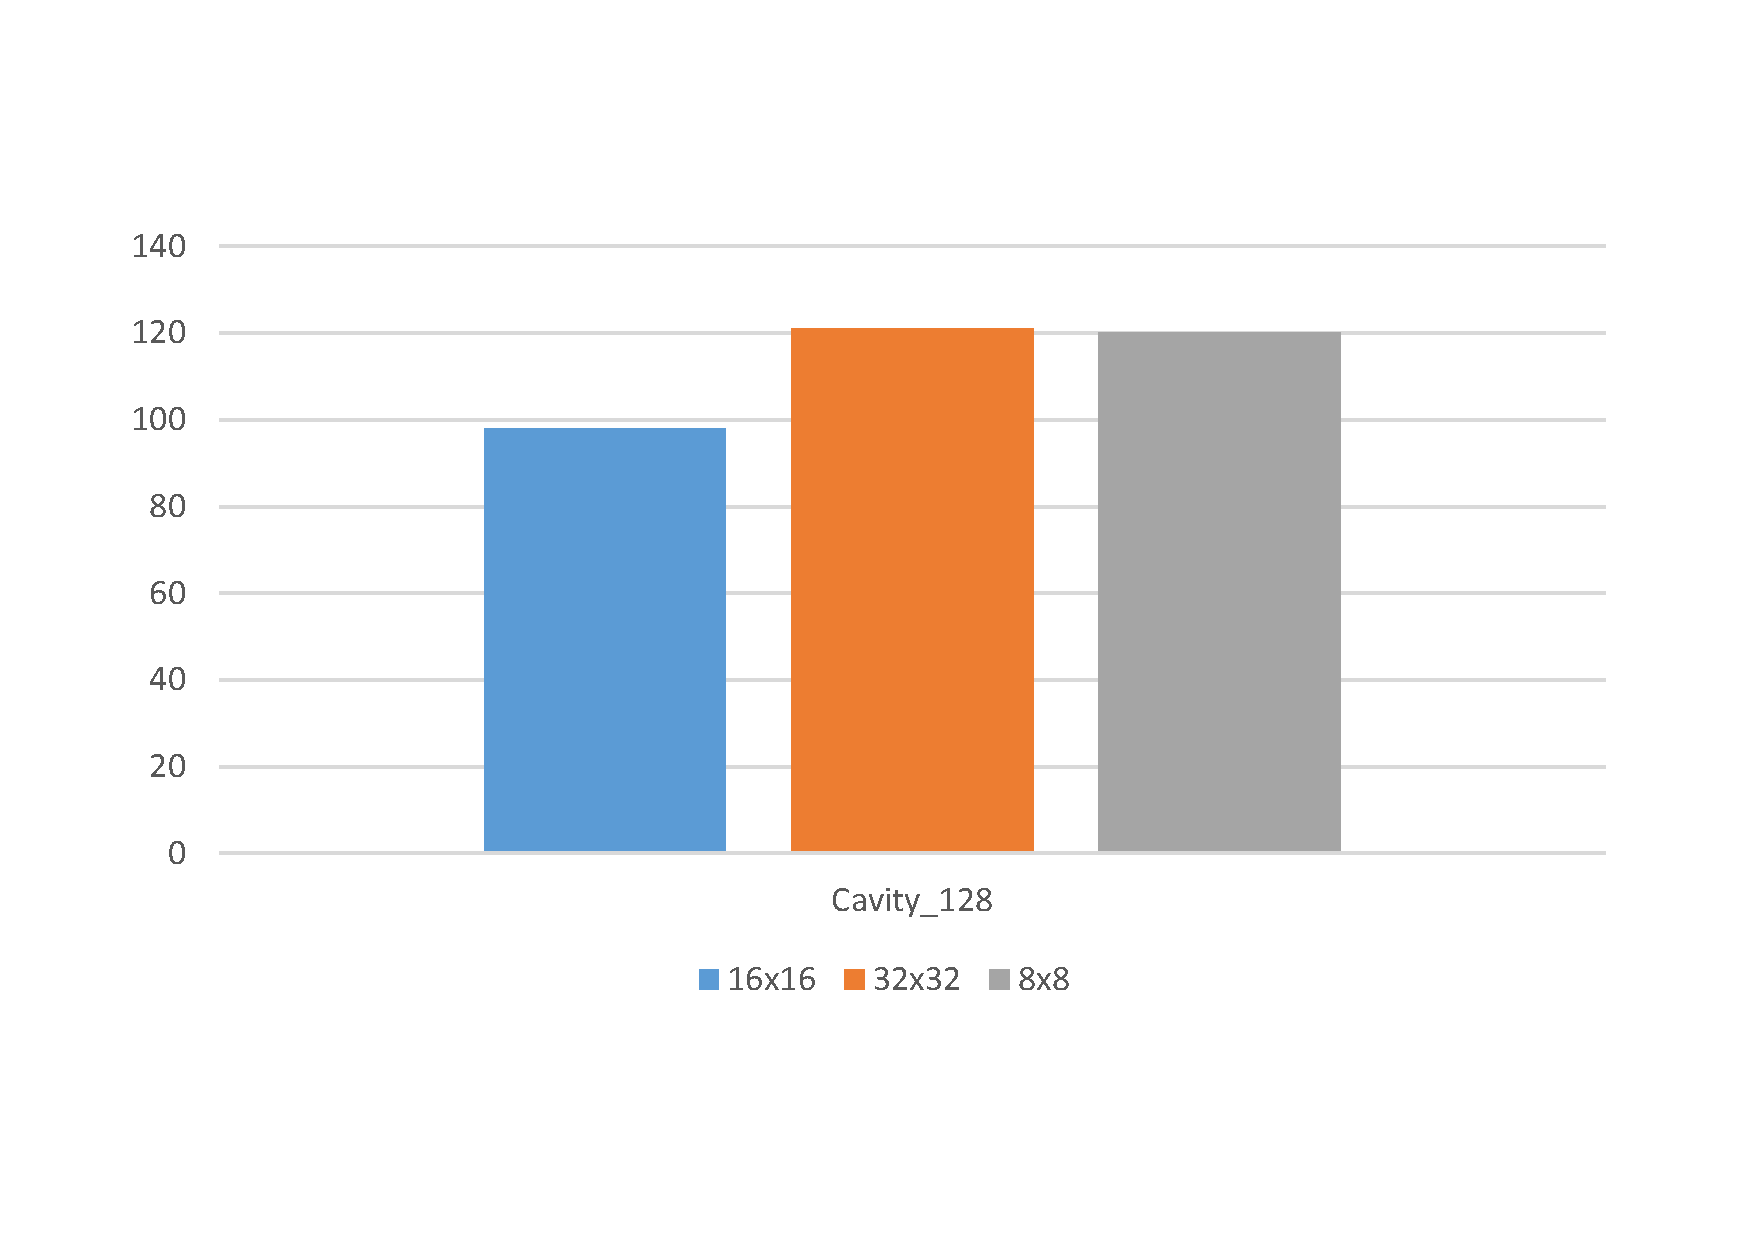
\includegraphics[width=\linewidth]{Resources/Images/timesThreads128.pdf}
		\caption{Cavity\_128}
	\end{subfigure}
	\begin{subfigure}{.49\textwidth}
		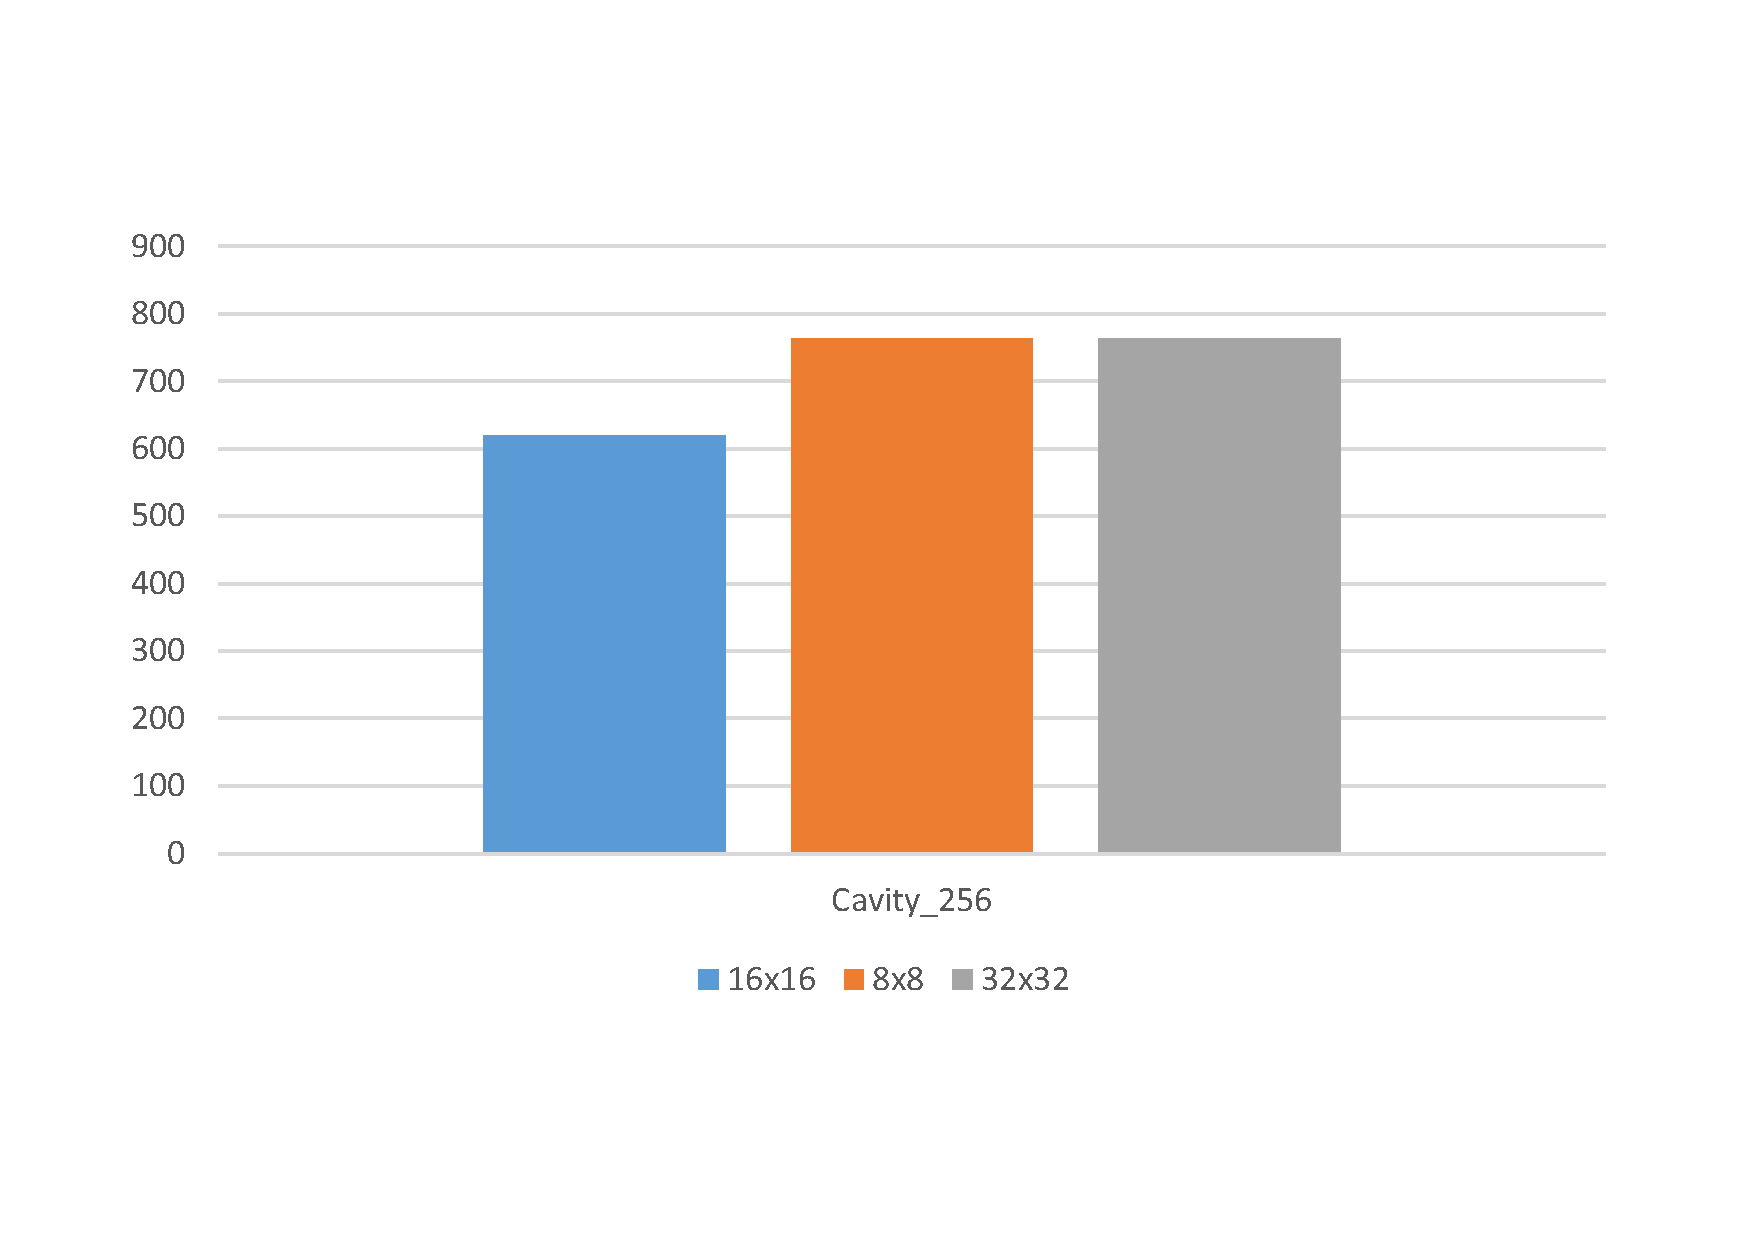
\includegraphics[width=\linewidth]{Resources/Images/timesThreads256.pdf}
		\caption{Cavity\_256}
	\end{subfigure} 
	\caption{Overall time comparison using three different threads per block configuration}
	\label{fig:timesThreads}
\end{figure} 

Figure \ref{fig:timesThreads} shows that the initial configuration (16x16) provides the best results. Because of this, the parallelisation strategy for the multiphase algorithm development will also start with this number of threads per block.


\subsection{Validation}
Now that the received code has been validated to perform under the same conditions as the final version used by the previous authors, we now have to verify whether the results that the received version is producing are the same as the final one. The validation of the results obtained throughout this project will be under the responsibility of Antonio González. As such, the details for this initial validation can be found in his thesis \cite{antonioThesis}.
\par This initial validation is essential for the development of a multiphase flow using the in-house solver. Without it, there would be no way of telling whether the solver would be functioning incorrectly due to a faulty algorithm implemented by us or if the solver was already producing wrong results. By doing so we can be sure that our code behaves correctly and that a proper result is achieved.

\section{Developing the Color Gradient model}
After making sure that the code we received was producing correct results, we could start implementing the Color Gradient (CG) model in the in-house LBM solver. Since there are two people working on this project, a proper separation of responsibilities  was vital for a successful adaption of the solver. To this end, Antonio González \cite{antonioThesis} was in charge of the physical aspects of the model whilst I was in charge of the software side. \par
We first decided to implement the CG model in a serial fashion so as to easily and quickly find potential errors in the code. Antonio would then develop a working script of the model in Matlab and, after validating it, I would take that script and patch it into the LBM solver. After making sure that the model was working in full integration with the LBM solver, I could then start parallelising the algorithms and finally validate the final, parallel results. We felt that this process, while extensive and time consuming, presented the best way of correctly implementing the model, since it was easier to track bugs, and so was repeated for the 3D model.
\subsection{Initial arguments}
The LBM solver depends on some initial parameters to initialize the required variables correctly. To do so, a SetUpData.ini file needs to be filled with the desired values. Figure \ref{fig:setupLBM} shows the initial arguments on which the LBM solver depends upon.

\begin{figure}[H]
	\centering
	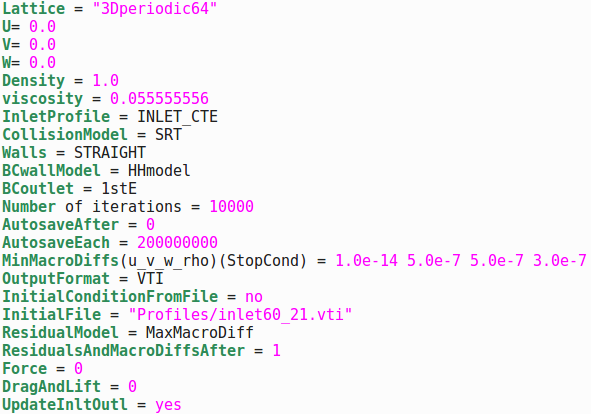
\includegraphics[width=0.9\linewidth]{Resources/Images/setup.png}
	\caption{Setup file for the LBM solver}
	\label{fig:setupLBM}
\end{figure}
 However, the CG model requires several additional parameters. These parameters had to be added to the solver and can be viewed in Fig. \ref{fig:setupCG}.
\begin{figure}[H]
	\centering
	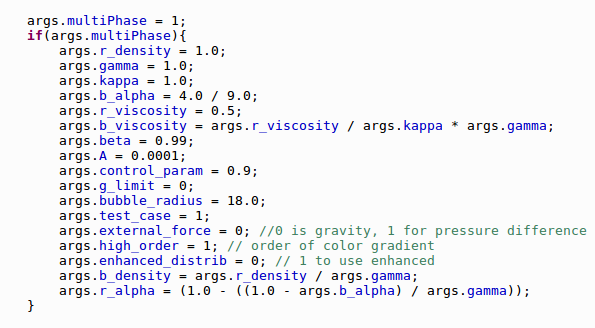
\includegraphics[width=0.9\linewidth]{Resources/Images/setupCG.png}
	\caption{Initial arguments for the Color Gradient model}
	\label{fig:setupCG}
\end{figure}

This model is supposed to be an addition to the original solver. As such, we need to keep the non-multiphase approach interchangeable with the new model. This was taken into account throughout the development of the code and so the user is provided with a way to easily switch between approaches. \par
The number of new parameters further shows how much the complexity of the solver will increase due to the new model. A higher complexity translates into more computations being performed, which in turn means that the CG model will hinder the original solver's performance. I will try to mitigate these effects during the parallelization of the solver, which I describe in more detail in Section \ref{sec:performance}. Also, two new distribution functions need to be added to the solver (one per fluid), as well as two new densities. All of this needs to be taken into account when developing the new solver.

\subsection{2D model}
After initializing all the parameters, we need to initialize the new distribution functions and the new densities. This is done depending on the test case to be used, where each distribution function and density array are initialized according to the initial parameters and to the region of the fluid. The test cases are explained in more detail in Section \ref{sec:testcases}. \par
As mentioned in Section \ref{sec:cgModel}, the Color Gradient model imposes some changes on the sub-steps of the LBM solver. The most noticeable of theses changes happen in the collision sub-step. First, we need to calculate the color gradient of each node. Since this color gradient is the result of a sum of interactions from the 9 directions of the speed model, we need a separate loop before being able to use this array in the computation of the perturbation operator. However, the color gradient calculation depends on the orientation of the node, that is whether the node is in the north, south, east, west or middle of the mesh. We can then calculate the appropriate collision frequency and afterwards compute the perturbation, collision and recoloring operators by looping between the 9 directions. For the most part of this sub-step, parallelization is implemented by following the example of the solver's previous collision sub-step. Each node will have it's own thread to perform calculations, and since each node does not depend on it's neighbors we do not have to worry about conflicted access to memory. However, each thread needs to know it's orientation for the color gradient calculation. Instead of having each thread reverse calculate it's index in an x,y format, a new array was created and initialized in the initialization section of the solver. This array has an element per node and it's value represents the orientation of the node in the following manner:
\begin{itemize}
	\item 1 - North
	\item 2 - South 
	\item 3 - East 
	\item 4 - West 
	\item 0 - Middle
	\item -1 - Corner    
\end{itemize}
This way each thread simply needs to access this array with it's index to discover which orientation it needs to take into account. \par
The streaming step behaves like the original solver's streaming. We now have to stream not just one distribution function but both of them, as each fluid's changes are specific to it's own function. However, the 2D model was not behaving correctly when nodes near the boundary needed to be updated. This could be fixed by analyzing the mesh interpolation and how the stream array is built, which specifies whether a direction of the speed model should be updated or not. Since there was not enough time to perform this analysis, I used the same array as the one used in the color gradient to find out the orientation of node. Then I simply needed to specify how the streaming should work for each orientation. \par
The boundary step also behaves like the original solver's boundary update. However, the tests used to validate the Color Gradient model mostly use periodic boundaries, which did not exist in the 2D version of the previous solver. As such, these boundaries needed to be implemented and added to the 2D version of the solver. Furthermore, the boundaries also need an interpolation of the mesh in order for each thread to know what type of boundary that node should be updated with. Since the lattice generator software was out of scope for this thesis, I again used the same array built with the orientations for the color gradient model. This way, each thread could identify which boundary condition should be applied depending on the position of the node. \par
The macro variable updates need to be replicated for both distribution functions and densities. Also, the calculation of the velocity needs to take both fluids into account. Other than that, it behaves in the same manner as the original solver. \par
Finally, the residuals calculation also needed to be updated since the previously implemented residuals based on the sum of absolute differences between each iteration's distribution function was not properly obeying the convergence criteria for our multiphase approach. Now, the residuals are based on the maximum difference of the distribution function and the user can choose which should the convergence criteria be in the setup file.    

\subsection{3D model}
The 3D model adaptation was much easier than the 2D implementation since for the most part it was just a matter of extending the computations on the distribution functions, from 9 to 19 directions. The core logic behind every operation was the same. However, the collision model needed to be updated since the collision frequencies, perturbation operator and equilibrium distribution function calculation were based on a enhanced version of the 2D model's version. Eventually we also modified the 2D version to use this enhanced collision step since it was meant to provide more accurate results. \par
One of the most significant improvements from implementing the 3D model was that the previous solver had more enhancements in 3D than in 2D. We could now use the proper streaming and boundary steps since there were no complications when generating 3D meshes and the software could adequately interpolate these meshes and initialize control arrays correctly. 

\section{Validation}
The validation of the results was performed by Antonio González \cite{antonioThesis}. To do so, every test case was implemented according to their specific needs. Almost every case was based on the same mesh, a simple square or cube depending on the dimension. The only exception was the Rayleigh-Taylor instability where a rectangular mesh was used. Appendix \textcolor{red}{Ref appendix validation} shows that the model produces correct results for every test case. \par
The solver has the option of producing results in different formats, .dat, .vti and .csv. .VTI files were the addition of last year's authors and can be read using Paraview \cite{paraview}. The main advantage of these files is that they require significantly less memory than the other formats. Because of this, we are able to save time by transferring the results from Cranfield's HPC center faster and also by making post-processing analysis less time consuming. For this reason, we extended the creation of these files to use the new multiphase model arrays.
\section{Test cases}\label{sec:testcases}
The validation of the CG model depends not only on the analysis of the actual result of the simulation, but also in the type of test case used. Each test case had different requirements in the software since they depended on different arrays and each used their own type of verification. Because of this, I added the option to change between test cases as an argument in the setup file. During the execution of the solver, this options allows for a correct initialization of the densities and distribution functions, as well as adequately storing information when needed.
A total of 6 test cases were implemented for the 2D model and 4 for the 3D model.
\subsection{Steady bubble} 
\begin{figure}[H]
	\centering
	\begin{subfigure}{.49\textwidth}
		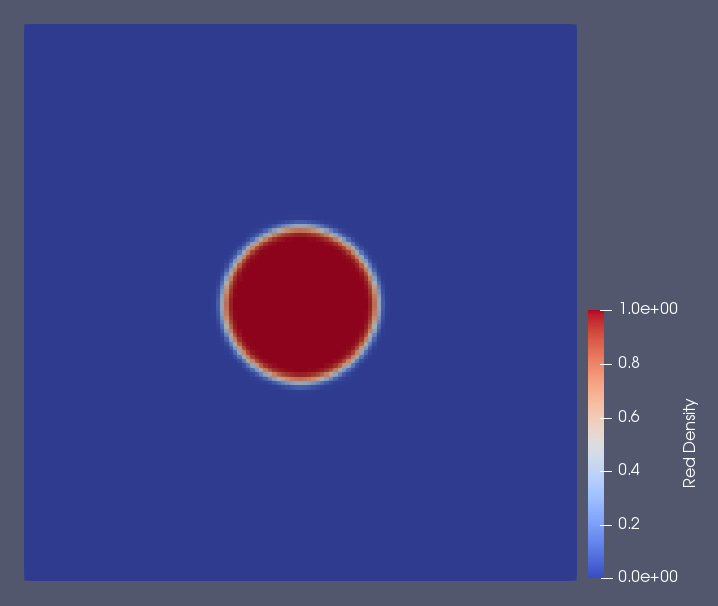
\includegraphics[width=\linewidth]{Resources/Images/steadyBubble.png}
		\caption{2D model}
	\end{subfigure}
	\begin{subfigure}{.49\textwidth}
		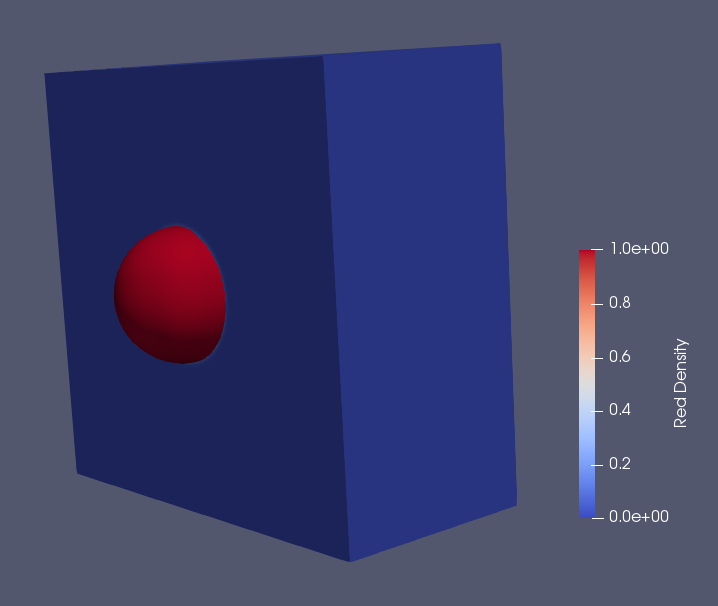
\includegraphics[width=\linewidth]{Resources/Images/steadyBubble3d.png}
		\caption{3D model}
	\end{subfigure} 
	\caption{Red fluid density for the Steady bubble case}
	\label{fig:steady}
\end{figure} 
This test aims to simulate a stationary bubble of an immiscible fluid inside another immiscible fluid. Although this test is the simplest physically, it is one the most computationally expensive tests to perform. To validate this test, we need to store the evolution of the surface tension over time. This entails calculating the pressure difference inside and outside the bubble, resulting in 4 additional reduce operations in every iteration. Reduce operations are very expensive in GPUs since these are operations that are dominated by memory access, requesting a heavy amount of memory access inside the GPU as well as when transferring information between the CPU and GPU. We are likely to see an increase in performance when running simulations with other, less computationally demanding test cases. 
\subsection{Deforming bubble}
\begin{figure}[H]
	\centering
	\begin{subfigure}{.49\textwidth}
		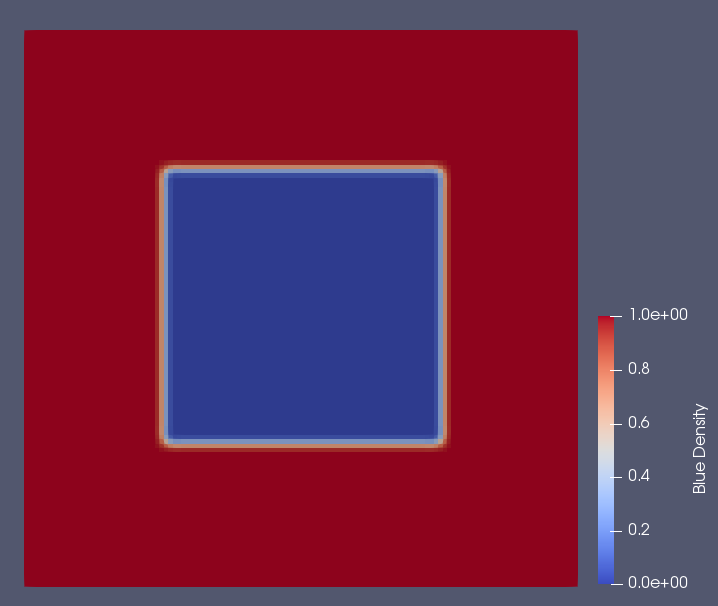
\includegraphics[width=\linewidth]{Resources/Images/square.png}
		\caption{2D model}
	\end{subfigure}
	\begin{subfigure}{.49\textwidth}
		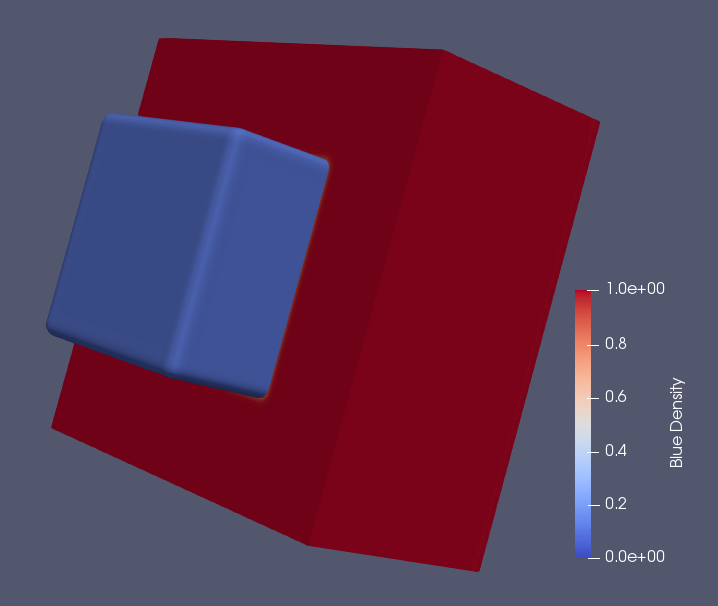
\includegraphics[width=\linewidth]{Resources/Images/square3D.png}
		\caption{3D model}
	\end{subfigure} 
	\caption{Blue fluid density for the deforming bubble case}
	\label{fig:deforming}
\end{figure} 
This test simulates a fluid that starts as a deformed bubble, a square, and eventually converges into a steady, stable bubble. This test is much less computationally expensive. The only verification needed is the difference between the final bubble radius and the predicted radius, which is only done once, at the end of the simulation.  

\subsection{Coalescing bubbles}
\begin{figure}[H]
	\centering
	\begin{subfigure}{.49\textwidth}
		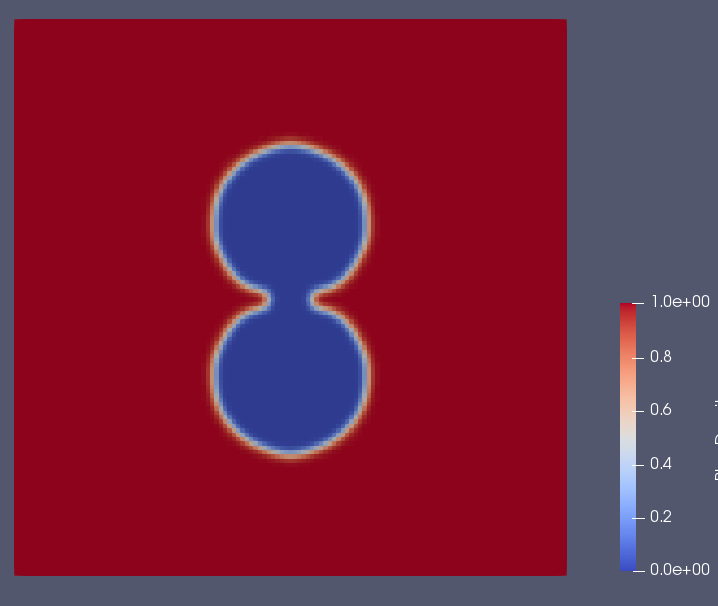
\includegraphics[width=\linewidth]{Resources/Images/coal.png}
		\caption{2D model}
	\end{subfigure}
	\begin{subfigure}{.49\textwidth}
		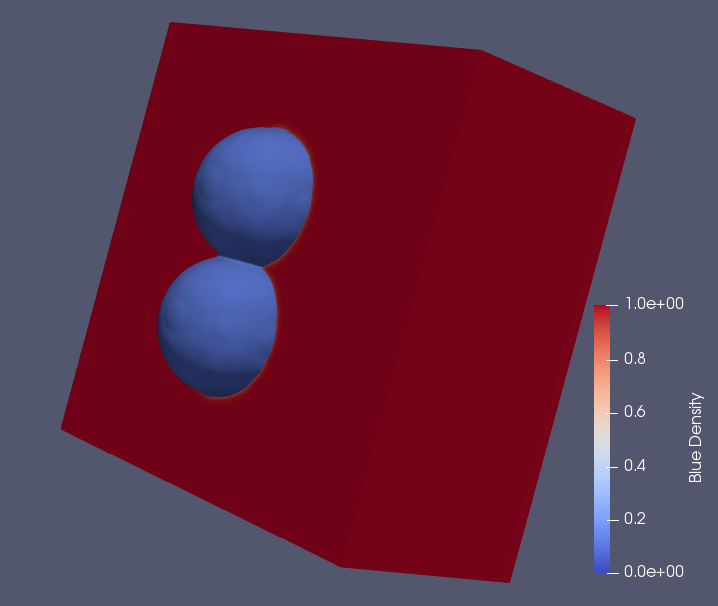
\includegraphics[width=\linewidth]{Resources/Images/coal3d.png}
		\caption{3D model}
	\end{subfigure} 
	\caption{Blue fluid density for the coalescing bubbles case}
	\label{fig:coalescence}
\end{figure} 
This test simulates the coalescence of two bubbles of the same fluid inside another fluid. The bubbles start by having only a small point of contact between each other and then eventually coalesce into a bigger, steady bubble. As was the case with the deforming bubble test, in this scenario we only need to compare the final radius of the bubble with a predicted one, making this test also less computationally demanding. 

\subsection{Oscillating bubble}
\begin{figure}[H]
	\centering
	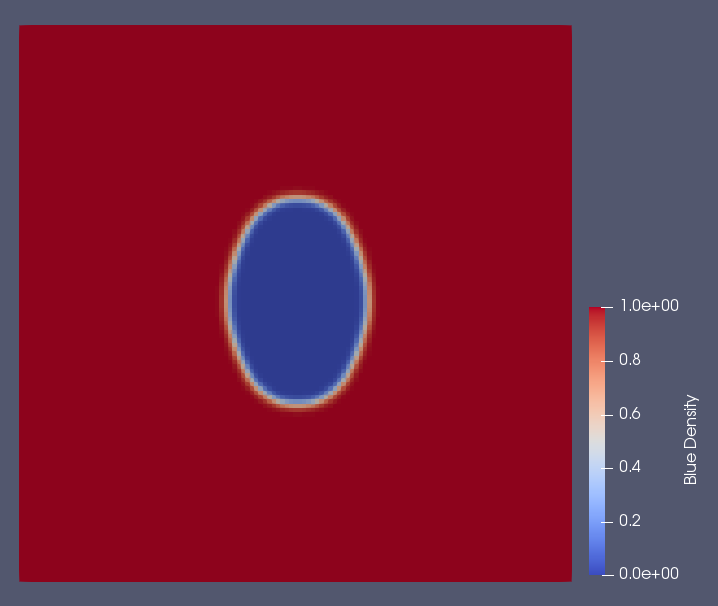
\includegraphics[width=0.9\linewidth]{Resources/Images/oscil.png}
	\caption{Blue fluid density for the 2D oscillating bubble}
	\label{fig:oscil}
\end{figure}
In this test, a bubble following an ellipsoid is created inside another fluid. The bubble then starts oscillating vertically and horizontally until it stabilizes into a steady bubble. For this test case, we need to find out the maximum height in y of the interface between the two fluids. This implies more computations and memory accesses per iteration which will hinder the solver's performance. This is needed so we can obtain a profile of the bubble's oscillation which will later be post-processed at the end of the simulation.  


\subsection{Couette flow}
\begin{figure}[H]
	\centering
	\begin{subfigure}{.49\textwidth}
		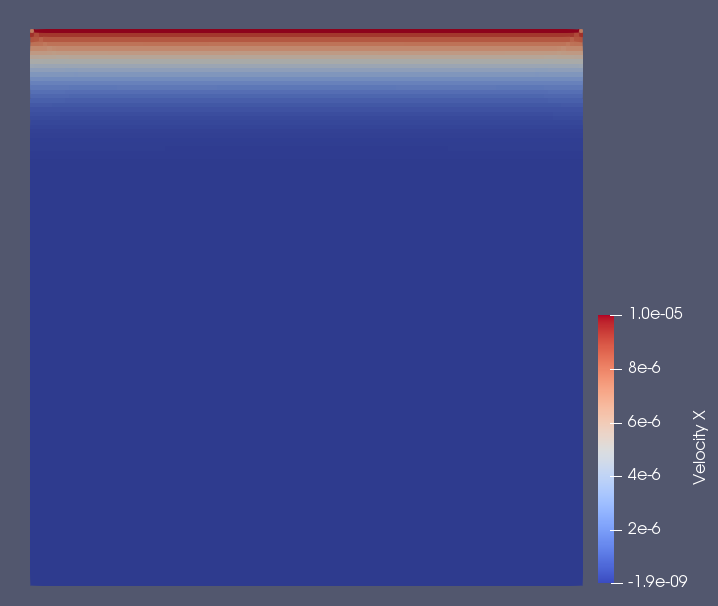
\includegraphics[width=\linewidth]{Resources/Images/couette.png}
		\caption{2D model}
	\end{subfigure}
	\begin{subfigure}{.49\textwidth}
		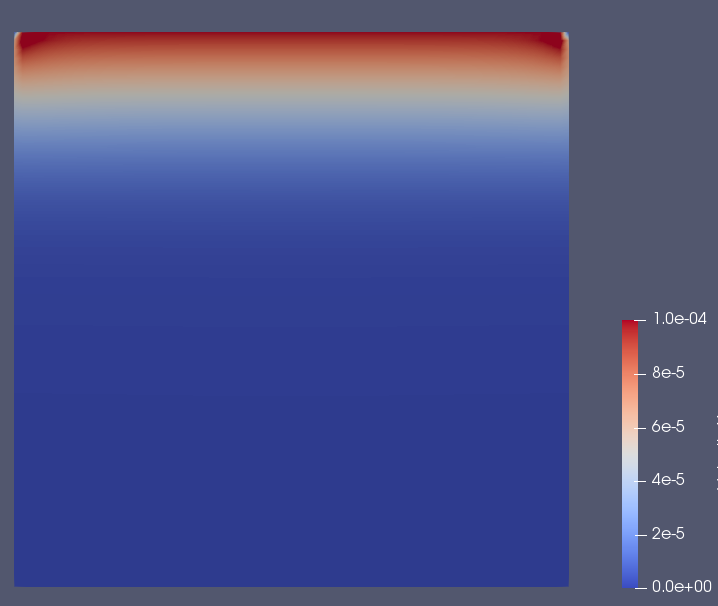
\includegraphics[width=\linewidth]{Resources/Images/couette3D.png}
		\caption{3D model}
	\end{subfigure} 
	\caption{X velocity with a few iterations using the Couette flow case.}
	\label{fig:couette}
\end{figure} 
All of the previous tests were not fully using all the initial parameters, they were tests where the external conditions were of no great importance. To fully test our new model, we decided to test conditions where the boundaries of the mesh were not all periodic, and so we decided to test the Couette flow. In this case, the north boundary is an inlet with a constant velocity in x, while the south boundary is a wall where the fluid bounces back from. Once again, this test is also less computationally demanding since we only need to verify the profile of the velocity once at the end of the simulation. 

\subsection{Rayleigh-Taylor instability}
\begin{figure}[H]
	\centering
	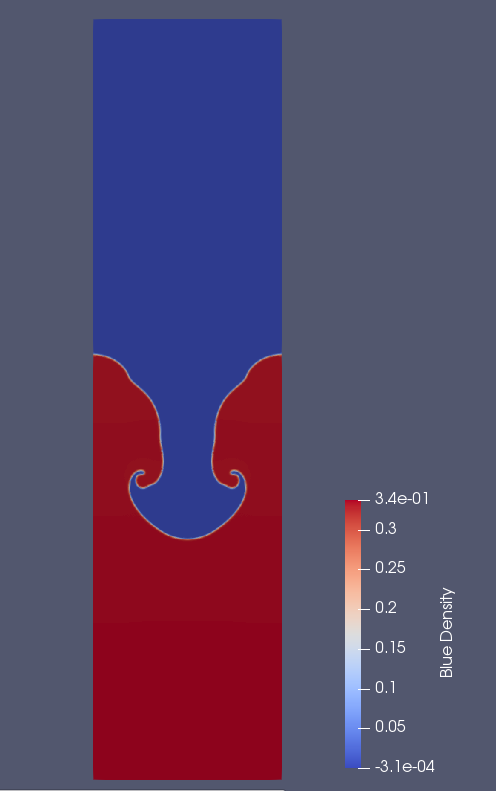
\includegraphics[width=0.5\linewidth]{Resources/Images/rt.png}
	\caption{Blue fluid density for the 2D Rayleigh-Taylor instability}
	\label{fig:rt}
\end{figure}
Finally, we chose to implement the Rayleigh-Taylor instability since in this test we can adequately test the functionalities of our CG model. Here, a heavy fluid is set on top of another, lighter fluid. Then the heavier fluid starts descending with the force of gravity and eventually starts creating vortices in the other fluid. The needs for this case are similar to the oscillating bubble case, but instead of calculating the maximum height of the interface we calculate the minimum. Because of the same memory access and number of computations, this is the third most computationally expensive test in the new LBM solver.

\section{Memory usage}
The amount of memory used is a crucial factor when performing large scale simulations. Even more so if we want the results to mimic real-word scenarios. For this reason, I have performed an analysis on the amount of memory that the new Color Gradient model requires on the LBM solver from the GPU. Tables \ref{tab:2dmem} and \ref{tab:3dmem} show the amount of memory used by the 2D and 3D mesh containing 128 nodes in each direction.
\begin{table}[H]
	\centering
	\begin{tabular}{|l|l|l|}
		\hline
		\textbf{Variables}              & \textbf{Variable size}   & \textbf{Memory (MB)} \\ \hline
		\textbf{Initialization}         & $3 * m * n$              & 0.1875               \\ \hline
		\textbf{BC initialization}      & $7 * N_{Conn}$           & 0.0399475098         \\ \hline
		\textbf{Macroscopic values}     & $9 * m * n$              & 0.5625               \\ \hline
		\textbf{Boundary conditions}    & $16 * N_{BC}$            & 0.0302734375         \\ \hline
		\textbf{Distribution functions} & $6 * 9 * m * n$          & 3.375                \\ \hline
		\textbf{Residuals}              & $3 * 9 * m * n$          & 1.6875               \\ \hline
		\textbf{Temporary values}       & $5 * m * n$              & 0.3125               \\ \hline
		\textbf{Temporary values 2}     & $8 * m * n $        	   & 0.5                    \\ \hline
		\textbf{Sum}                    &                          & ~6.7         \\ \hline
	\end{tabular}	
	\caption{2D memory usage for Cavity 128 with Single precision}
	\label{tab:2dmem}
\end{table}

For the 2D model, we see that the solver requires a small amount of memory, which is normal since a 128x128 is considered a coarse mesh for 2D problems. We could easily increase the number of nodes computed without affecting the required memory in a significant manner. 

\begin{table}[H]
	\centering
	\begin{tabular}{|l|l|l|}
		\hline
		\textbf{Variables}              & \textbf{Variable size}   & \textbf{Memory (MB)} \\ \hline
		\textbf{Initialization}         & $4 * m * n * h$          & 32                   \\ \hline
		\textbf{BC initialization}      & $8 * N_{Conn}$           & 14.953125            \\ \hline
		\textbf{Macroscopic values}     & $9 * m * n * h$          & 72                   \\ \hline
		\textbf{Boundary conditions}    & $3 * N_{BC}$             & 0.0115356445         \\ \hline
		\textbf{Distribution functions} & $6 * 19 * m * n * h$     & 912                  \\ \hline
		\textbf{Residuals}              & $3 * 19 * m * n * h$     & 456                  \\ \hline
		\textbf{Temporary values}       & $5 * m * n * h$          & 40                   \\ \hline
		\textbf{Temporary values 2}     & $18 * m * n * h$         & 144                  \\ \hline
		\textbf{Sum}                    &                          & ~1562.964      \\ \hline
	\end{tabular}
	\caption{3D memory usage for Cavity 128 with Single precision}
	\label{tab:3dmem}
\end{table}

In the 3D model, the memory usage is on a completely different scale. We now see that for the same mesh as in Table \ref{tab:2dmem}, extended to another direction, the used memory increases approximately 233 times. This makes the memory used by the 2D model almost insignificant when compared with the 3D version.\par
To further analyze what this increase in memory means, I have prepared Table \ref{tab:memCG} showing the different memory requirements for both single and double precision and comparing between a 128 and 256 sized mesh.

\begin{table}[H]
	\centering
	\begin{tabular}{|c|c|c|c|}
		\hline
		\textbf{Type}    & \textbf{Nodes} & \textbf{Single precision} & \textbf{Double precision} \\ \hline
		\textbf{2D\_128} & 16384          & 6.32                      & 11.7                      \\ \hline
		\textbf{2D\_256} & 65536          & 24                        & 46.57                     \\ \hline
		\textbf{3D\_128} & 2097152        & 1563                      & 3026                      \\ \hline
		\textbf{3D\_256} & 16777216       & 12336                     & 24054                     \\ \hline
	\end{tabular}
	\caption{Memory usage for the Color Gradient model in MB}
	\label{tab:memCG}
\end{table}

We can now clearly see how the memory used by the solver is one of the most important aspects to take into account. In fact, the memory requirements are so big in some cases (for the 3D, 256 sized mesh) that we cannot test the solver against this type of mesh since the maximum available global memory in a Cranfield's GPU is 11440 MBytes. \par
There were some ways to decrease this memory requirement. We could eliminate one of the distribution functions (and add more calculations to compensate) or change the residuals calculation to be based on the macroscopic variables instead of the distribution function. However, we found that these changes would imply a decrease in the solver's accuracy and stability, for which we chose to not implement these "improvements" in the final version of the solver.

\section{Performance of the parallel code}\label{sec:performance}
In this section, we will analyze and discuss the performance obtained throughout the various stages of development of the code. We will first compare optimizations techniques employed, followed by the usage of different code and compiler features. We will then compare the different hardware used and finally the impact in performance between using double and single precision. 
\subsection{GPU specification}
To perform the tests, we first need the hardware on which to perform the tests on. Since we are using CUDA, we must obviously use machines with NVIDIA GPUs. Table \ref{tab:specs} shows the specification of the characteristics of each machine's GPU. GRID and Delta are a part of Cranfield's HPC center, while the laptop is my own personal laptop with a less powerful GPU.
\begin{table}[H]
	\centering
	\begin{tabular}{|l|c|c|c|}
		\hline
		\multicolumn{1}{|c|}{\textbf{}} & \textbf{GRID} & \textbf{Delta} & \textbf{Personal laptop} \\ \hline
		\textbf{GPU}                    & Tesla K40m    & Tesla K80      & GeForce GTX 850M         \\ \hline
		\textbf{Memory}                 & 12288 MB      & 11440 MB       & 4044 MB                  \\ \hline
		\textbf{CUDA capability}        & 3.5           & 3.7            & 5.0                       \\ \hline
		\textbf{CUDA cores}             & 2880          & 2496           & 640                      \\ \hline
		\textbf{GPU clock rate}         & 745 MHz       & 824 MHz        & 902 MHz                  \\ \hline
		\textbf{Mem. clock rate}        & 3004 MHz      & 2505 MHz       & 1001 MHz                 \\ \hline
	\end{tabular}
	\caption{Specification of the used GPUs}
	\label{tab:specs}
\end{table}
\subsection{2D model}
\subsubsection{Normal distribution function v1.0}
\subsubsection{Enhanced distribution function v2.0}
\subsubsection{Optimizations v2.1}
\subsubsection{Loop unrolling v2.2}
\subsubsection{Final version v2.3}
\subsubsection{High order color gradient}
\subsubsection{CUDA compute capability}
\subsection{3D model}
\subsubsection{Enhanced distribution function v1.0}
\subsubsection{Final version v1.1}
\subsubsection{High order color gradient}
\subsubsection{CUDA compute capability}
\subsection{Hardware}
\subsection{Double vs Single}
\chapter{Conclusions}

%% Back matter
%
% This is where we include appendices and references

\appendix

\bibliography{AllBib}{}
\bibliographystyle{plain}
\end{document}